\documentclass[12pt]{report}
\usepackage{graphicx}
\usepackage{amsmath}
\usepackage{amsfonts}
\usepackage{amssymb}
\usepackage[english]{babel}
\usepackage[utf8]{inputenc} 
\usepackage[T1]{fontenc} 
\usepackage{lmodern} 
\usepackage{hyperref} 
\usepackage{lscape} 
%\usepackage{subfigure} 
\usepackage{multirow}
\usepackage{graphicx}
\usepackage[parfill]{parskip}  
\usepackage{makeidx}
%\usepackage{ucs}
%\DeclareUnicodeCharacter{00A0}{~}
\newcommand{\captionfonts}{\it}
\makeatletter
\long\def\@makecaption#1#2{%
\vskip\abovecaptionskip
\sbox\@tempboxa{{\captionfonts #1: #2}}%
\ifdim \wd\@tempboxa >\hsize
{\captionfonts #1: #2\par}
\else
\hbox to \hsize{\hfill\box\@tempboxa\hfill}%
\fi
\vskip\belowcaptionskip}
\makeatother

%%%%%%%%%%%%%%%%%%%%%%%%%%%%%%%%%%%%%%%%%%%%%%%%%%%%%%%%%%%%%%%%%%%%%%%%
%DEFINITIONS
%%%%%%%%%%%%%%%%%%%%%%%%%%%%%%%%%%%%%%%%%%%%%%%%%%%%%%%%%%%%%%%%%%%%%%%

\def\be{\begin{equation}}
\def\ee{\end{equation}}



%\def\bea{\begin{eqnarray}}
%\def\eea{\end{eqnarray}}
%\def\deu{{\delta}^{(1)}}
%\def\ded{{\delta}^{(2)}}
%\def\de3{{\delta}^{(3)}}
\def\H{\,{\mathcal  H}}
%\def\cal H{\,{\mathcal  H}}
%\def\calm{{\cal M}}
%\def\calp{{\cal P}}
%\def\calr{{\cal R}}
%\newcommand\bfa{{\bf a}}
%\newcommand\bfb{{\bf b}}
%\newcommand\bfc{{\bf c}}
%\newcommand\bfd{{\bf d}}
%\newcommand\bfe{{\bf e}}
%\newcommand\bff{{\bf f}}
%\newcommand\bfg{{\bf g}}
%\newcommand\bfh{{\bf h}}
%\newcommand\bfi{{\bf i}}
%\newcommand\bfj{{\bf j}}
%\newcommand\bfk{{\bf k}}
%\newcommand\bfl{{\bf l}}
%\newcommand\bfm{{\bf m}}
%\newcommand\bfn{{\bf n}}
%\newcommand\bfo{{\bf o}}
%\newcommand\bfp{{\bf p}}
%\newcommand\bfq{{\bf q}}
%\newcommand\bfr{{\bf r}}
%\newcommand\bfs{{\bf s}}
%\newcommand\bft{{\bf t}}
%\newcommand\bfu{{\bf u}}
%\newcommand\bfv{{\bf v}}
%\newcommand\bfw{{\bf w}}
%\newcommand\bfx{{\bf x}}
%\newcommand\bfy{{\bf y}}
%\newcommand\bfz{{\bf z}}
%\newcommand{\fNLl} {f_{\rm NL}^{\rm local}}
%\newcommand{\fNLe} {f_{\rm NL}^{\rm equil}}
%\newcommand{\fNLo} {f_{\rm NL}^{\rm ortog}}
%
%\newcommand{\fNL}  {f_{\rm NL}^{}}
%\newcommand{\LL}{{\mathrm{L}}}
%\newcommand{\NL}{{\mathrm{NL}}}


%\def\Aa{\frac{a^{\prime}}{a}}
%\def\Ab{\Big(\frac{a^{\prime}}{a}\Big)^2}
%\def\Ac{\frac{a^{\prime\prime}}{a}}
%\def\Dp{\delta^{(1)}}
%\def\Ds{\delta^{(2)}}
%\def\La{\partial_i \,\partial^i}
%\def\LA{\partial_k \,\partial^k}
%\def\deu{{\delta}^{(1)}}
%\def\ded{{\delta}^{(2)}}
%\def\ze{{1}^{(0)}}
%\def\wpsi{\widetilde{\Psi}}
%\def\simlt{\stackrel{<}{{}_\sim}}
%\def\simgt{\stackrel{>}{{}_\sim}}
%\def\R{{\mathcal R}}
%\def\S{{\mathcal S}}
%\def\C{{\mathcal C}}
%\def\P{{\mathcal P}}
%\def\B{{\mathcal  B}}
%\def\T{{\mathcal  T}}
%\def\La{\nabla^2}
%\def\LA{\nabla^2}
%\def\Q{{\mathcal Q}}
%\def\k{{\mathbf k}}
%\def\l{{\ell}}
%\def\d{{\rm d}}

%\usepackage{natbib} 
\makeindex
\date{}                                           

\includeonly{intro,chapter1,chapter2,chapter3,chapter4,chapter5,
chapter6,chapter7,chapter8,chapter9}

\begin{document}
\renewcommand{\figurename}{\textbf{Fig.}}
\renewcommand{\tablename}{\textbf{Tab.}}

\thispagestyle{empty}
\begin{center}  

\Large  \textbf{Title} \\
  
\vspace{4cm}  

\large Ph. D. Thesis

\vspace{4cm}

submitted at the Department of Theoretical Physics \\

of the \\

UNIVERSITY OF GENEVA\\

to obtain the degree of \\

\textit{Docteur ès Sciences, mention Physique}\\

by\\

\large \textbf{Wilmar A. Cardona}\\  

\vspace{4cm} 

\large Thesis N. \\  
\normalsize 2016  

\end{center}  

\newpage  
\pagenumbering{roman}
  
  
\vspace{6cm}  
\begin{center}

\large \textit{To ...}
\normalsize

\end{center}
  
\newpage  

\addcontentsline{toc}{section}{Acknowledgements}  
\chapter*{Acknowledgements} 

\vspace{3mm}

I would like ...
  
\newpage  

\addcontentsline{toc}{section}{Abstract}  
\chapter*{Abstract}  

\vspace{3mm}

Some important points ...

\newpage

\tableofcontents

\listoffigures

\listoftables 

\newpage

\pagenumbering{arabic}


\addcontentsline{toc}{chapter}{Introduction}
\chapter*{Introduction}
\label{intro} 

The $20$th century gradually saw the emergence of the standard model of cosmology. A linear relation between distances and recession velocities of galaxies \cite{Hubble:1929ig}, the observed abundance of chemical elements in the universe \cite{Gamow:1946eb,Alpher:1948ve,Gamow:1949zz,Alpher:1950zz}, and the existence of the Cosmic Microwave Background radiation (CMB) \cite{Alpher:1950zz,Penzias:1965wn} evidenced a dynamical rather than static universe: the universe is expanding. Observations of type Ia supernovae in $1998$ \cite{Riess:1998cb,Perlmutter:1998np} modified a ``little bit'' the picture, setting one of the most important problems cosmologists will be addressing in the $21$st century: the universe is not only expanding, it is speeding up and cosmologists want to find out why. 

The cosmological principle -- the assumption that the universe at sufficiently large scales is homogeneous and isotropic -- is one of the cornerstones of the concordance model of cosmology \cite{Robertson:1935zz,Walker1937}. If one assumes there is no charge asymmetry in the universe \cite{Caprini:2003gz}, the only relevant interaction on large scales is gravity. In the vanilla model of cosmology the gravitational interaction is described by Einstein's General Relativity. Solutions for Einstein's field equations -- that couple geometry to both matter-energy and pressure -- satisfying the cosmological principle are known the since early $20$th century \cite{Friedman:1922kd,Friedmann:1924bb,Lemaitre:1927zz,Lemaitre:1931zz}. In those solutions -- the so-called FLRW metric -- the expansion of the universe is given by the scale factor $a(t)$, a function which depends on the cosmic time $t$ and scales the distance between two given points as the universe expands. The matter content in the standard model of cosmology is only partially given by particles in the Standard Model (SM) of particle physics (i.e., photons, electrons, and so on). The remaining matter, dubbed Cold Dark Matter (CDM) because it only seems to interact with the baryonic matter through gravity, is required, for instance, to fit observations of galaxy velocities in galaxy clusters \cite{Zwicky:1933gu}. Finally, in order to describe the accelerated expansion of the universe, the concordance model of cosmology reintroduces the cosmological constant $\Lambda$ (first introduced by Albert Einstein in the early $20$th century). The standard model of cosmology is thus named  $\Lambda CDM$ model.

The universe is obviously not completely homogeneous since inhomogeneities exist, such as galaxies and clusters of galaxies. Moreover, both the convergence of observations into a flat universe and the fact that the CMB appears to be incredibly uniform in regions now causally disconnected  make the $\Lambda CDM$ model an incomplete description of the universe. These three main difficulties of the standard model of cosmology (i.e., structure formation, horizon, flatness) can be solved by adding an inflationary epoch to the history of the universe \cite{Guth:2005zr}. In the simplest inflationary scenarios the potential energy of a scalar field drives an exponential expansion in the very early universe rendering the universe extremely flat very quickly (within about $10^{-35}\, \second$). The universe would have evolved from a tiny patch (about $10^{-26}\,\mathrm{m}$) where regions that are today are causally isolated were then in causal contact thus solving the horizon problem of the standard model of cosmology. Perhaps most importantly, inflationary models predict that quantum fluctuations of the scalar field in the early stage of the universe would have seeded the density fluctuations we observe today in the form of galaxies, galaxy clusters, and CMB fluctuations.

Over the past three decades cosmology has witnessed the come of an age of precision. Full sky CMB experiments such as Cosmic Background Explorer (COBE) \cite{Smoot:1992td}, Wilkinson Microwave Anisotropy Probe (WMAP) \cite{Bennett:2003bz}, and PLANCK satellite \cite{Ade:2013sjv} have measured CMB anisotropies in different frequencies and on a wide range of angular scales thus allowing a careful study of the predictions made by the inflationary $\Lambda CDM$ model. The CMB spectrum matches incredibly well that of a black body with temperature $2.7\,\mathrm{K}$ as predicted by the standard model \cite{Alpher:1950zz}. By investigating CMB fluctuations cosmologists have been able to constraint to high accuracy the curvature of the universe: it agrees pretty well with the flatness prediction of inflationary models \cite{Ade:2015xua}. Although rather controversial, there is no compelling evidence for significant deviations of the cosmological principle in the Planck CMB data \cite{Ade:2015hxq}. Furthermore, current CMB experiments support the existence of dark matter and also the accelerated expansion of the universe. Galaxy surveys such as Sloan Digital Sky Survey (SDSS) have also played an important role in testing cosmological models \cite{Tegmark:2003uf,Tegmark:2003ud}. Partially mapping the distribution of mass in the universe, using observations of $\approx 10^6$ galaxies with mean red shift $z \approx 0.1$, SDSS collaboration detected a baryon acoustic peak which is an imprint of the recombination-epoch acoustic oscillations on the low-redshift clustering of matter \cite{Eisenstein:2005su}. This detection confirms a prediction of the standard cosmological theory. Upcoming galaxy surveys offer thus an important complementary probe and will be key for testing cosmological models in the near future, for instance to determine the neutrino mass.

The current concordance cosmological model, although both simple and a good fit for current data sets, lacks in fundamental grounds. On the one hand, it assumes the existence of dark matter which thus far has not been directly observed; the only known dark matter candidate being neutrinos. On the other hand, the cosmological problem poses a serious conundrum for quantum field theory which is unable to explain the extremely tiny observed value of the vacuum energy. Numerous alternative approaches to explain the accelerated expansion of the universe from first principles have been proposed over the past years. In one family of models evolving scalar fields -- easily found in fundamental theories of matter -- have been used to model dark energy as a fluid driving the late-time acceleration \cite{Copeland:2006wr}. Another family of models exploits the ambiguity of the cosmological constant in the Einstein field equations and proposes that modifications of General Relativity -- the theory of gravity in the concordance model -- could be the reason that accounts for the speeding up of the universe \cite{Clifton:2011jh}. Therefore although remarkable progress has been made on both theory and observation, degeneracies at the model level\footnote{The situation is even worst taking into account the number of inflationary scenarios which are compatible with current observations. Although non-Gaussianity of CMB fluctuations was expected to break the degeneracy in inflationary models, the 2015 Planck results \cite{Ade:2015ava,Ade:2015lrj} showed that there are still several inflationary models compatible with observations.} are still present and efficient ways to discriminate cosmological models are needed.   

In Chapter \ref{chapter-ade} of this thesis Lukas Hollenstein, Martin Kunz and I have considered one possibility for breaking degeneracies at the model level. Dark energy anisotropic stress is a key feature as it allows to discriminate the standard dynamical dark energy model -- a scalar field minimally coupled to gravity-- from the so-called modified gravity models. In linear theory, the former class of models does not support any anisotropic stress whereas models such as scalar-tensor and $f(R)$ generically have a non-zero anisotropic stress. We have adopted a phenomenological approach and studied a model of anisotropic dark energy which encompasses both internally and externally sourced anisotropic stress, that additionally allows for a scale dependence \cite{Cardona:2014iba}. In particular, we have investigated how the presence of a non-zero dark energy anisotropic stress impacts both the dark matter and dark energy perturbations, as well as CMB angular power spectrum. We found approximate solutions for both dark matter and dark energy perturbations in some particular scenarios and constrained dark energy anisotropic stress parameters with recent data sets. 

Gleaning information about cosmological parameters from all the available data sets will surely shed light on the shortcomings of the $\Lambda CDM$ model. Indeed, upcoming galaxy surveys such as Dark Energy Survey \href{www.darkenergysurvey.org}{(DES)}, Dark Energy Spectroscopic Instrument \href{http://desi.lbl.gov/}{(DESI)}, Large Synoptic Survey Telescope \href{www.lsst.org}{(LSST)}, Physics of the Accelerating Universe Survey \href{www.pausurvey.org}{(PAUS)}, and \href{www.euclid-ec.org}{EUCLID} will play a key role in understanding the accelerated expansion of the universe and constraint the neutrino masses. The come of all this new data will make necessary very careful analyses and appropriate modelling of the statistical properties of the matter density field. In particular, since those galaxy surveys will probe scales comparable to the horizon, analyses must properly include relevant relativistic effects. In Chapter \ref{chapter-mnu} of this thesis, Ruth Durrer, Martin Kunz, Francesco Montanari and I have investigated the impact of neglecting lensing convergence when analysing data from a EUCLID-like survey. We have shown that neglecting lensing convergence when constraining neutrino masses, for instance, would lead to spurious detection of their absolute mass scale, thus hindering one of the key foals of future surveys \cite{Cardona:2016qxn}. Moreover, we found that since biases of cosmological parameters in analyses neglecting lensing might reach several standard deviations, the usual linear approximation in Fisher matrix formalisms breaks down,  therefore it might no longer be appropriate. We have then adopted a Markov Chain Monte Carlo (MCMC) approach to yield reliable forecasts.

Reliable, accurate, model independent measurements of the Hubble constant $H_0$ are essential to understand the physics behind the phenomenologically successful $\Lambda CDM$ model. Accurate and precise determinations of $H_0$ will make possible to put tighter constraints on dark energy parameters -- such as the equation of state for dark energy $w$ -- and the mass of neutrinos. Although direct measurements of $H_0$ have proven to be difficult (e.g., control of systematic errors, relatively small data sets, fully consistency of different methods for measuring distances), remarkable progress has been achieved over past decades; improvements include an enlarged sample of $\SNe$ hosts having a Cepheid calibrated distance, reduction of uncertainties on anchor distances, and increase of infra-red observations of Cepheid stars. All these efforts have yielded a direct $H_0$ measurement almost as precise as the indirect determination for the $\Lambda CDM$ model derived by the Planck collaboration \cite{Ade:2015xua,Riess:2016jrr}. The group led by Adam Riess has recently found a $H_0$ value which is in a $\approx 3\sigma$ disagreement with that derived from CMB measurements \cite{Riess:2016jrr}. The reasons underlying this tension are unclear (e.g., remaining CMB systematics, issues with utilised statistical methods), but if the disagreement is proved robust, it might signify new physics.  In Chapter \ref{chapter-h0} of this thesis, Martin Kunz, Valeria Pettorino, and I have developed a statistical method using Bayesian hyper-parameters to measure the Hubble constant with the available data. The method allows a comprehensive treatment of the available data sets with no need for arbitrary outlier rejection algorithms. Our measurement of $H_0$ is a bit less precise than that by Riess et al. \cite{Riess:2016jrr}, but we understand this as a result of inconsistencies in the data sets. 

\chapter{Standard model of cosmology}
\label{chapter:1} 

\section{Introduction}
\label{section:1.1}

One can hardly imagine a bigger and more complex  physical system than the universe. Questions like ``How did we get here ?'' and  ``When did the universe start ?'' have been addressed in different epochs by different cultures and by different means during mankind history. The scientific and technological development of last century has allowed scientists from different fields (e.g., physics, astronomy and mathematics) to achieve a remarkable progress in the understanding of the universe. 

Cosmologists still have to give a satisfactory answer to the fundamental questions referenced above. Nevertheless, investigating the universe over the last decades, we have accumulated some experience in the field and new and  sophisticated questions have come out: why is the universe speeding-up ? is there a new kind of energy with negative pressure ? or instead should we look for a new theory of gravity ? how did the structures we see in the universe (e.g., galaxies, clusters of galaxies) form ? what is dark matter ? 

Those questions have motivated the development of new theories, which in turn, have been the building blocks of innovative cosmological models. Unfortunately, this wonderful theoretical work have brought us to a point where different models can reproduce our current cosmological observations, that is, our space of models presents degeneracies. Luckily, not only the theoretical cosmology has seen progress. People working on observational cosmology also have been following a successful path, being awarded some Nobel prizes already.  The new instruments are looking at the universe much more farther than $50$ years ago and with an amazing precision. Hopefully, the new generation of satellites and surveys will help to falsify some cosmological models and break the existing degeneracies.

In this Chapter we will introduce the simplest cosmological model, also known as concordance model or $\Lambda$CDM.  It will also allow us to specify the notation that we will use in the thesis. 

As an starting point we could ask ourselves the following questions concerning the system we aim to study:

\begin{enumerate}
\item Which are the components of the universe ?
\item Where does the content of the universe act ? N-dimensional space-time ? is it continuous or discrete ?  does it change with time ?
\item Which  are the interactions governing the components of the universe ? what is their energy scale and range ? how well do we know these interactions ? to which extent are they valid ? Which are the theories we use to describe them ?
%\item How can we build models of the universe ? 
\item How can we test those models ? which kind of experiments and observations do we use ? 
\end{enumerate}

In the coming sections we will try to explain how those questions are addressed in the Standard model of cosmology. 

 %However, before going on let us discuss briefly a few points about the construction of models of the universe. So far we have identified some considerations before In order to build models of the universe we should: 

%\begin{enumerate}
%\item choose a period of time where the laws of physics are relatively well-known and tested
%\item identify which are the relevant components present during the period (which might be different along the way)
%\item define where those components act (which might be change as time evolves) 
%\item make assumptions or considerations about relevant interactions during the chosen period
%\item Finally, try to build the model according to the items above
%\end{enumerate}

%After building the models we can test whether they correspond to what we see or not. 

%I will try to address the questions above in order to introduce the standard model of cosmology

How is this chapter organised ?

\section{Matter $+$ Fundamental interactions}
\label{section:1.2}

It is known that matter is constituted by particles that have different properties (e.g., mass, charge, spin). Moreover, particles interact with each other in different ways depending on their particular properties. According to our current understanding of nature there are four fundamental interactions, namely: gravity, weak interaction, strong interaction and electromagnetic interaction. Gravity is described by the General Theory of Relativity (hereafter GR) whereas the other three fundamental interactions are described by the standard model of particle physics (hereafter SM). These two descriptions of the fundamental interactions are probably the two most outstanding achievements in modern physics so far. 

\begin{table}
\begin{tabular}{|c|c|c|}
\hline   & Energy scale (GeV) & Length scale \\ 
\hline  CMB &  $ 10^{-10} $ & $ \sim 10^{29} \times \ell_p $\\ 
\hline  Electroweak phase transition & $ 10^3 $ & $ \sim 10^{16} \times \ell_p $\\ 
\hline  LHC & $ 10^4 $ & $ \sim 10^{15} \times \ell_p $\\ 
\hline  GUT & $ 10^{16} $ & $ \sim 10^3 \times \ell_p $\\ 
\hline  Planck scale & $ 10^{19} $ & $ \ell_p $\\ 
\hline 
\end{tabular}
\caption{Key energy scale}
\label{table:1}
\end{table}

I must compare data in Table \ref{table:1} with the size of the universe in the corresponding epochs.


In spite of the great success of both GR and SM, there are some caveats with these two descriptions of nature. On one hand, there is not quantum counterpart for GR which is important in a model of the very early universe. On the other hand, SM does not account for neutrino oscillations and dark matter which is a key ingredient in the standard model of cosmology. 
  
In the $\Lambda$CDM model the components of the universe are divided as follows. There are mainly three type of constituents, namely: 

\begin{itemize}
\item the cosmological constant $\Lambda$;
\item the cold dark matter (CDM) and the baryonic matter (non-relativistic matter);
\item the radiation (relativistic matter).
\end{itemize}

There is a huge mismatch between the value of the cosmological constant computed within the SM and that deduced from cosmological observations. This is known as the cosmological constant problem. On the other hand, cosmological observations have shown that the amount of matter needed to fit, for instance, rotational speeds of galaxies, must be bigger than what the amount of matter accounted for the baryonic matter. This missing matter seems to be constituted by particles moving slower than the speed of light and only interacts with SM particles through gravity. Not explanation has been given neither for the cosmological constant problem nor for the nature of the dark matter so far. 

\texttt{This kind of answers the first and third questions above. However, I should add a figure for the regime of validity of the interactions and explain things much more better. Then, I must focus on the description of the geometry. Papers by A. G. Walker and H. Robertson may be helpful}

One of the cornerstones of the $ \Lambda $CDM model of cosmology is the cosmological principle. It claims that our universe is homogeneous and isotropic in scales $ \sim 100 h^{-1} $ Mpc. The universe is modelled by a $ 4- $dimensional manifold. It can be shown that in such a manifold the most general metric fulfilling the requirements of the cosmological principle is the well-known FLRW metric,


\begin{equation}
ds^2=-dt^2+a^2(t)\left[\frac{dr^2}{1-K r^2}+r^2d\Omega^2\right] \, , 
\label{equation:1.2.1}
\end{equation}

where

\begin{equation}
d\Omega^2=d\theta^2+\sin^2\theta d\phi^2 \, ,
\label{equation:1.2.2}
\end{equation}

is the metric of the unit sphere, $ r,\, \theta,\,\phi $ are comoving coordinates, $ t $ is the cosmic time, $ a(t) $ is the scale factor, and $ K $ is a curvature constant for $ 3- $dimensional hyper-surfaces: $ K=1,\, -1,\, 0 $ for spherical, hyperbolic, and flat geometries, respectively. The FLRW metric can also be written as  

\begin{equation}
ds^2=-dt^2+a^2(t)\left[d\chi^2+f(\chi)^2d\Omega^2\right] \, ,
\label{equation:1.2.3}
\end{equation}

where the relation between $ r $ and $ \chi $ is given by

\begin{equation}
r=f(\chi)=\left \{\begin{array}{lll} \sin\chi & \longrightarrow & K=1\\
\chi & \longrightarrow & K=0\\
\sinh\chi & \longrightarrow & K=-1\end{array}\right \} \, .
\label{equation:1.2.4}
\end{equation}

If we consider a radial trajectory for a photon emitted at $ (t,\chi) $ and detected at $ (t_0, 0) $, we can use the metric \eqref{equation:1.2.3} along with $ ds=0 $ to find

\begin{equation}
\chi=\int_t^{t_0}{\frac{dt}{a(t)}} \, .
\label{equation:1.2.5}
\end{equation}

Let us consider two consecutive crests in an electromagnetic wave. If we consider that the scale factor $ a(t) $ is approximately constant during a period of the wave, we find   

\begin{equation}
\frac{\lambda_0}{\lambda_1}=\frac{a_0}{a_1} \, ,
\label{equation:1.2.6}
\end{equation}

where $ \lambda_0 $ and $ \lambda_1 $ are the wavelengths of the observed wave and of the emitted wave, respectively; $ a_0\equiv a(t_0) $ and $ a_1 \equiv a(t) $ refer to the scale factor at detection and emission, respectively. 

Defining the red-shift as 

\begin{equation}
z \equiv \frac{\lambda_0}{\lambda_1}-1 \, ,
\label{equation:1.2.7}
\end{equation}

we can write the equation \eqref{equation:1.2.6} as a relation between the red-shift $ z $ and the scale factor $ a $

\begin{equation}
z+1=\frac{a_0}{a_1} \, .
\label{equation:1.2.8}
\end{equation}

The scale factor is a pretty important function because, as we will see later on, it gives us information about the expansion history of the universe. Assuming that $ a(t) $ is an analytical function, it can be Taylor expanded 

\begin{equation}
a(t)=a_0\left \{1+\frac{t-t_0}{t_H}-\frac{q_0}{2}\left(\frac{t-t_0}{t_H}\right)^2+\dots\right \} \, ,
\label{equation:1.2.9}
\end{equation}

where

\begin{equation}
t_H \equiv \frac{a(t_0)}{\dot{a}(t_0)} \, ,
\label{equation:1.2.10}
\end{equation}

is called the Hubble time and

\begin{equation}
q_0 \equiv -\left[\frac{a\ddot{a}}{\dot{a}^2}\right]_{t_0} \, ,
\label{equation:1.2.11}
\end{equation}

is the deceleration parameter.\footnote{Hereafter we will denote derivatives with respect to the cosmic time $ t $ by a dot, for instance, $ \dot{a} = \dfrac{d a}{d t}$.} From equation \eqref{equation:1.2.11} we can see that when $ q_0<0 $ the universe is speeding up, that is, $ \ddot{a}>0 $.

We can also define the Hubble parameter 

\begin{equation}
H(t)\equiv \frac{\dot{a}}{a} \, ,
\label{equation:1.2.12}
\end{equation}

which allow us to rewrite the Hubble time $ t_H $ as

\begin{equation}
t_H = H^{-1}(t_0) \, .
\label{equation:1.2.13}
\end{equation}
 
To finish this section we define the particle horizon $ r_{max}(t) $ which will be important when reviewing the inflationary paradigm in Chapter \ref{chapter:2}. Let us consider a ray light emitted at  $ (t=0,\,r=0) $ travelling towards an observer receiving the signal at time $ t $. With a FLRW metric \eqref{equation:1.2.1} the greatest  radial distance $ r_{max}(t) $ from which the observer can be aware of is given by 
 
\begin{equation}
\int_0^t \frac{dt'}{a(t')} = \int_0^{r_{max}(t)} \frac{dr}{\sqrt{1-K r^2}} \, .
\label{equation:1.2.14}
\end{equation} 

The physical distance corresponding to the particle horizon would be given by 

\begin{equation}
d_{max}(t) = a(t) \int_0^{r_{max}(t)} \frac{dr}{\sqrt{1-K r^2}} = a(t) \int_0^t \frac{dt'}{a(t')} \, .
\label{equation:1.2.15}
\end{equation} 


\section{Dynamics}
\label{section:1.3}

Since cosmology aims at investigating the universe, it is necessary to determine which are the fundamental interactions we should take into account. Nowadays, we are aware of four fundamental interactions: weak, strong, electromagnetic, and gravitational. Weak and strong interactions are irrelevant beyond distances of order $ 10^{-15} $ m and $ 10^{-16} $ m, respectively. The distances considered by the cosmological principle are of order $ 10^{24} $ m, therefore both weak and strong interactions are negligible in a cosmological context. 

On the other hand, there is no observational evidence of neither electrical charges nor electrical currents at cosmological scales. Since those are the sources of the electromagnetic field, we can, in principle, disregard the electromagnetic interaction. 

As a result, the only fundamental interaction to be considered is gravity. The most successful theory for describing gravitation is the Einstein General Theory of Relativity. According to this theory, there exists a relation between the space-time geometry and its energetic content. In order to describe the energetic content of the universe, we employ the energy-momentum tensor of a perfect fluid which reads 

\begin{equation}
T_{\mu\nu}=P g_{\mu\nu} + (P+\rho)U_{\mu}U_{\nu}  \qquad \text{ou} \qquad  T^{\mu}_{\nu}=diag(-\rho, P, P, P) \, ,
\label{equation:1.3.1}
\end{equation}        

with $ g_{\mu\nu} $ being the space-time metric, and $ P $, $ \rho $, $ U_{\mu} $ the pressure, the density and the $ 4- $velocity of the fluid, respectively. An ideal fluid whose pressure is a function only of the density, $ P=P(\rho) $, is called a barotropic fluid. In the standard model of cosmology it is assumed that the energetic components of the universe are ideal, barotropic fluids whose equation of state can be written as

\begin{equation}
P = w \rho \, ,
\label{equation:1.3.2}
\end{equation}

where $ w $ is a constant: $ 1/3 $ for radiation, $ 0 $ for non-relativistic matter; if $ w<-1/3 $ the fluid is usually referred as dark energy.

The connections $ \Gamma^\alpha_{\beta\gamma} $ of the metric $ g_{\mu\nu} $ are defined as  

\be
\Gamma^\alpha_{\beta\gamma}\,\equiv \,
\frac{1}{2}\,g^{\alpha\rho}\left( \frac{\partial
g_{\rho\gamma}}{\partial x^{\beta}} \,+\, \frac{\partial
g_{\beta\rho}}{\partial x^{\gamma}} \,-\, \frac{\partial
g_{\beta\gamma}}{\partial x^{\rho}}\right)\, .
\label{equation:1.3.3}
\ee

which in turn allow us to define the Riemann tensor

\be
R^{\alpha}_{~\beta\mu\nu}=
\Gamma^{\alpha}_{\beta\nu,\mu}-\Gamma^{\alpha}_{\beta\mu,\nu}+
\Gamma^{\alpha}_{\lambda\mu}\Gamma^{\lambda}_{\beta\nu}-
\Gamma^{\alpha}_{\lambda\nu}\Gamma^{\lambda}_{\beta\mu} \,,
\label{equation:1.3.4}
\ee

the Ricci tensor -- a contraction of the Riemann tensor \eqref{equation:1.3.4} -- 

\begin{equation}
R_{\mu\nu}\,\equiv \, \partial_\alpha\,\Gamma^\alpha_{\mu\nu} \,-\,
\partial_{\mu}\,\Gamma^\alpha_{\nu\alpha} \,+\,
\Gamma^\alpha_{\sigma\alpha}\,\Gamma^\sigma_{\mu\nu} \,-\,
\Gamma^\alpha_{\sigma\nu} \,\Gamma^\sigma_{\mu\alpha}\, ,
\label{equation:1.3.5}
\end{equation}

and the Ricci scalar -- a contraction of the Ricci tensor --

\begin{equation}
R \equiv g^{\mu\alpha}\,R_{\alpha\mu}= R^{\mu}_{~\mu} \, .
\label{equation:1.3.6}
\end{equation}

The Einstein equations for an universe whose matter content is described by a perfect fluid \eqref{equation:1.3.1} read 


\begin{equation}
G_{\mu\nu} = \kappa^2 T_{\mu\nu} - \Lambda g_{\mu\nu} \qquad ; \qquad \kappa^2 \equiv \frac{8\pi}{M_p^2} \quad ; \quad M_p^2 \equiv  \frac{1}{G} \, ,
\label{equation:1.3.7}
\end{equation}

where $ \Lambda $ is the cosmological constant, $ M_p $ is the Planck mass, and $ G_{\mu\nu} $ is the Einstein tensor defined as 

\begin{equation}
G_{\mu\nu} \equiv R_{\mu\nu} - \frac{1}{2}g_{\mu\nu}R \, .
\label{equation:1.3.8}
\end{equation}

The Einstein equations \eqref{equation:1.3.7} stablish a relation between the matter content in the universe (left hand side) and its geometry (right hand side). If we define the energy-momentum tensor for a cosmological constant as

\begin{equation}
T_{\mu\nu}^{vac} \equiv -\frac{\Lambda g_{\mu\nu}}{\kappa^2} \, ,
\label{equation:1.3.9}
\end{equation}

the equation \eqref{equation:1.3.7} can be rewritten as

\begin{equation}
G_{\mu\nu} = \kappa^2 T_{\mu\nu} \, ,
\label{equation:1.3.10}
\end{equation}

where $ T_{\mu\nu} $ is the total energy-momentum tensor, that is, the sum of all the matter contributions including the cosmological constant.

From the time-time component of the Einstein equations \eqref{equation:1.3.10} we can obtain one of the key equations in the $ \Lambda $CDM model, namely, the Friedman equation 

\begin{equation}
H^2=\left(\frac{\dot{a}}{a}\right)^2=\frac{\kappa^2 \rho}{3}-\frac{K}{a^2}\, ,
\label{equation:1.3.11}
\end{equation}

where $ \rho $ and $ K $ are the total energy density and the curvature constant, respectively. From the space-space components of equation \eqref{equation:1.3.10} along with the Friedman equation \eqref{equation:1.3.11} it is straightforward to find the acceleration equation (also called Raychaudhuri equation) 

\begin{equation}
\left(\frac{\ddot{a}}{a}\right)=-\frac{\kappa^2 }{6}\left(\rho+3P\right) \, .
\label{equation:1.3.12}
\end{equation}

On the other hand, if we use the identity 

\begin{equation}
\dot{H}=\frac{\ddot{a}}{a}-H^2 \, ,
\label{equation:1.3.13}
\end{equation}

along with the Friedman equation \eqref{equation:1.3.11} in the acceleration equation \eqref{equation:1.3.12}, we can write  

\begin{equation}
\dot{H}=-\frac{\kappa^2}{2} (\rho+P)+\frac{K}{a^2} \, .
\label{equation:1.3.14}
\end{equation}
 
Let us define the parameter density $ \Omega_i $ for each sort of matter as 
 
\begin{equation}
\Omega_i (t)\equiv \frac{\rho_i(t)}{\rho_c(t)}\, ; \qquad \rho_c \equiv \frac{3H^2}{\kappa^2} \, ; \qquad \rho_{\Lambda} \equiv \frac{\Lambda}{\kappa^2} , 
\label{equation:1.3.15}
\end{equation}

$ i $ being an index indicating different kinds of matter, $ \rho_c $ the critical density, and $ \rho_{\Lambda} $ the energy density of a cosmological constant. The Friedman equation \eqref{equation:1.3.11} can be written as taking the form 

\begin{equation}
\Omega_{Tot}(t)-1=\frac{K}{a^2H^2(t)},
\label{equation:1.3.16}
\end{equation}

where

\begin{equation}
\Omega_{Tot} (t) = \sum_i \Omega_i \, .
\label{equation:1.3.17}
\end{equation}

%%%%%%%%%%%%%%
%%%%%%%%%%%%%%
%%%%%%%%%%%%%%

\begin{table}[h!]
\centering
\begin{tabular}{|c|c|c|}
\hline
Density    & Curvature & Geometry \\ \hline
$\Omega_{Tot}>1$   & $K=1$     & spherical \\ \hline
$ \Omega_{Tot}=1 $ & $ K=0 $   & flat  \\ \hline
$ \Omega_{Tot}<1 $ & $ K=-1 $  & hyperbolic \\ \hline
\end{tabular}
\caption{Relation between density parameter and geometry.}
\label{table:1.3.1}
\end{table}

\begin{equation}
2R^{\alpha}_{\sigma;\alpha}-R_{;\sigma}=0 \, ,
\label{equation:1.3.18}
\end{equation}

\begin{equation}
T^{\mu}_{\nu;\mu} =0  \, ,
\label{equation:1.3.19}
\end{equation}

\begin{equation}
\dot{\rho}+3H(\rho+P)=0 \, .
\label{equation:1.3.20}
\end{equation}

\begin{equation}
\rho_i = \rho_{0i} a^{-3 (1+w)}; \qquad \left \{
\begin{array}{lll}w =1/3 & \longrightarrow & \rho_{\gamma} \propto a^{-4}\\
w=0 & \longrightarrow & \rho_M \propto a^{-3}\\
w =-1 & \longrightarrow & \rho_{\Lambda}(a)=\rho_{\Lambda}(a_0)\end{array}\right \} \, ,
\label{equation:1.3.21}
\end{equation}

\begin{equation}
a(t) \propto (t-t_0)^{\frac{2}{3(1+w)}}\, .
\label{equation:1.3.22}
\end{equation}

\begin{equation}
w <-1/3 \, ,
\label{equation:1.3.23}
\end{equation}
 
\begin{equation}
a(t) \propto e^{Ht} \, ,
\label{equation:1.3.24}
\end{equation}

\section{Comparison with observations}
\label{section:1.4}

\begin{equation}
\frac{d \mathfrak{R}}{dt}=H_0\mathfrak{R}+v_p \, ,
\label{equation:1.4.1}
\end{equation}

\begin{equation}
\Omega_{Tot} = \Omega_{\gamma} + \Omega_M + \Omega_{\Lambda} \approx 1 \, ,
\label{equation:1.4.2}
\end{equation}

\begin{equation}
\Omega_M + \Omega_{\Lambda} = 1 \, ,
\label{equation:1.4.3}
\end{equation}

\section{Shortcomings of the standard model}
\label{section:1.5}

\subsection{Flatness}
\label{subsection:1.5.1}

\begin{equation}
\frac{\ddot{a}}{a} = -\frac{1}{2}H^2 \Omega_{Tot} (1+3 w) \, .
\label{equation:1.5.1}
\end{equation}

\begin{equation}
\dfrac{d \Omega_{Tot}}{d \ln a} = (1+3 w)\Omega_{Tot} (\Omega_{Tot} - 1) \, .
\label{equation:1.5.2}
\end{equation}

\begin{equation}
\Omega_{Tot} (x) = \frac{1}{1-\alpha \exp^{(1+3 w)x}} \qquad ; \qquad x \equiv \ln a \, ,
\label{equation:1.5.3} 
\end{equation}   
 
\begin{equation}
\dfrac{d |\Omega_{Tot} - 1 |}{d x} > 0 \qquad se \qquad (1+ 3 w) > 0 \, ,
\label{equation:1.5.4}
\end{equation}   

\begin{equation}
w < -\frac{1}{3}\, ,
\label{equation:1.5.5}
\end{equation}

\begin{equation}
\dfrac{d |\Omega_{Tot} - 1 |}{d x} < 0 \,,
\label{equation:1.5.6}
\end{equation}

\begin{equation}
R_k^2 \equiv \frac{a^2}{|K|}\, ,
\label{equation:1.5.7}
\end{equation}

\begin{equation}
R_k^2 = \frac{1}{H^2 |\Omega_{Tot} -1 |} \, .
\label{equation:1.5.8}
\end{equation}

\begin{equation}
R_k^2 (t_0) \gg \frac{1}{H_0^2}\, .
\label{equation:1.5.9}
\end{equation}

\subsection{Horizon}
\label{subsection:1.5.2}

\begin{equation}
ds^2=a^2(\tau)\left[-d\tau^2 + \left[\frac{dr^2}{1-K r^2}+r^2d\Omega^2\right]\right]\, ,
\label{equation:1.5.10}
\end{equation} 


\begin{equation}
d\tau \equiv \dfrac{dt}{a(t)}\, .
\label{equation:1.5.11}
\end{equation}

\begin{equation}
d_H (t) = \int_0^t \frac{dt'}{a(t')} = \int_0^{\tau} d\tau' = \tau \, .
\label{equation:1.5.12}
\end{equation}

\begin{equation}
\tau \propto -\frac{1}{a H} \, .
\label{equation:1.5.13}
\end{equation}

\begin{equation}
\left( \frac{\lambda}{d_H}\right)^2 |\Omega - 1 |=const. \, .
\label{equation:1.5.14}
\end{equation}

\begin{equation}
\dfrac{d (\frac{\lambda}{d_H})}{dx} < 0\, .
\label{equation:1.5.15}
\end{equation}

\begin{equation}
\dfrac{d | \Omega_{Tot} - 1 |}{d x} < 0 \qquad se \qquad (1+ 3 w) < 0\, ,
\label{equation:1.5.16}
\end{equation}   

\begin{equation}
\dfrac{d (\frac{\lambda}{d_H})}{dx} > 0\, ,
\label{equation:1.5.17}
\end{equation}

\subsection{Another drawbacks}
\label{subsection:1.5.3}



\chapter{The inflationary paradigm}
\label{chapter:2}

\section{Introduction}
\label{section:2.1}

\section{The inflaton}
\label{section:2.2}

\begin{equation}
\ddot{a(t)}>0 \qquad \rightarrow \qquad \rho + 3 P < 0 \, ,
\label{equation:2.2.1}
\end{equation}

\begin{equation}
R_{CH} \equiv \frac{R_H}{a} = (aH)^{-1} \, ,
\label{equation:2.2.2} 
\end{equation} 

\begin{equation}
R_H = H^{-1} \, ,
\label{equation:2.2.3}
\end{equation}
 
\begin{equation}
\dfrac{dR_{CH}}{dt} = \dfrac{d (aH)^{-1}}{dt} < 0 \, .
\label{equation:2.2.4}
\end{equation}

\begin{equation}
S_{total} = \int d^4 x \sqrt{-g} \left( \frac{1}{2 \kappa^2} f(R) + L_{\varphi} \right) \, ; \quad \kappa^2 \equiv 8\pi G\, ,
\label{equation:2.2.5}
\end{equation}

\begin{equation}
L_{\varphi} = F(\varphi , g^{\mu\nu}\partial_{\mu} \varphi \partial_{\nu} \varphi) - V(\varphi) \, ,
\label{equation:2.2.6}
\end{equation}

\begin{equation}
f(R)=R \, ,
\label{equation:2.2.7}
\end{equation}

\begin{equation}
F(\varphi , g^{\mu\nu}\partial_{\mu} \varphi \partial_{\nu} \varphi)=-\frac{1}{2} g^{\mu \nu} \partial_{\mu} \varphi \partial_{\nu} \varphi \, ,
\label{equation:2.2.8}
\end{equation}

\begin{equation}
S_{total} = \int d^4 x \sqrt{-g} \left( \frac{1}{2 \kappa^2} R -\frac{1}{2}g^{\mu \nu} \partial_{\mu} \varphi \partial_{\nu} \varphi - V(\varphi) \right) \, .
\label{equation:2.2.9}
\end{equation}

\begin{equation}
\ddot{\varphi} + 3 H \dot{\varphi} + \dfrac{d V}{d \varphi} = 0 \, ,
\label{equation:2.2.10}
\end{equation}

\begin{equation}
\ddot{x} + \beta \dot{x} + \omega_0^2 x = 0 \, ,
\label{equation:2.2.11}
\end{equation}

\begin{equation}
3 H \dot{\varphi}\, ,
\label{equation:2.2.12}
\end{equation}

\begin{equation}
T_{\mu \nu} = \partial_{\mu}\varphi \partial_{\nu}\varphi - g_{\mu \nu} \left( \frac{1}{2}g^{\alpha \beta} \partial_{\alpha}\varphi \partial_{\beta}\varphi + V(\varphi) \right) \, .
\label{equation:2.2.13} 
\end{equation}

\begin{equation}
T^0_0 = -\rho_{\varphi} \qquad ; \qquad \rho_{\varphi} = \frac{1}{2}\dot{\varphi}^2 + V(\varphi) \, ,
\label{equation:2.2.14}
\end{equation} 

\begin{equation}
T^1_1 = P_{\varphi} \qquad ; \qquad P_{\varphi} = \frac{1}{2}\dot{\varphi}^2 - V(\varphi) \, .
\label{equation:2.2.15}
\end{equation}

\begin{equation}
w_{\varphi} \equiv \frac{P_{\varphi}}{\rho_{\varphi}} = \frac{\dot{\varphi}^2 - 2 V(\varphi)}{\dot{\varphi}^2 + 2 V(\varphi)} \, .
\label{equation:2.2.16}
\end{equation}

\section{Slow-roll conditions}
\label{section:2.3}

\begin{equation}
V(\varphi) \gg \dot{\varphi}^2 \qquad \longrightarrow \qquad P_{\varphi} \simeq -\rho_{\varphi} \qquad \longrightarrow \qquad w_{\varphi} \simeq -1 \, ,
\label{equation:2.3.1} 
\end{equation}

\begin{equation}
E = \frac{1}{2}\dot{x}^2 + V(x) \, ,
\label{equation:2.3.2}
\end{equation} 

\begin{equation}
V(x) \gg \frac{1}{2}\dot{x}^2 \, ,
\label{equation:2.3.3}
\end{equation}

\begin{equation}
E \approx V(x)\, ,
\label{equation:2.3.4}
\end{equation}

\begin{equation}
\rho_{\varphi} \approx V(\varphi)\, .
\label{equation:2.3.5}
\end{equation}

\begin{equation}
\frac{1}{2}\dot{x}^2 \, \rightarrow \, 0 \quad \mathrm{ou} \quad \dot{x} \, \rightarrow \, 0 \, .
\label{equation:2.3.6}
\end{equation}

\begin{equation}
\ddot{x} \ll 1 \, ,
\label{equation:2.3.7} 
\end{equation}

\begin{equation}
\ddot{\varphi} \ll 1 \, ,
\label{equation:2.3.8}
\end{equation}

\begin{equation}
H^2 = \frac{\kappa^2}{3}\left( \frac{1}{2}\dot{\varphi}^2 + V(\varphi) \right) \qquad \longrightarrow \qquad H^2 \simeq \frac{\kappa^2}{3}V(\varphi) \, ,
\label{equation:2.3.9}
\end{equation}

\begin{equation}
3 H \dot{\varphi} + \dfrac{d V}{d \varphi} \simeq 0 \, .
\label{equation:2.3.10}
\end{equation}
 
\begin{equation}
9 H^2 \dot{\varphi}^2 \simeq V'^2 \qquad \rightarrow \qquad H^2 V \gg V'^2 \qquad \rightarrow \qquad \frac{V'^2}{V} \ll H^2 \, .
\label{equation:2.3.11}
\end{equation}

\begin{equation}
\left( \frac{V'}{V}\right)^2 \ll 1 \, .
\label{equation:2.3.12}
\end{equation}

\begin{equation}
H^2 V \gg V'^2 \qquad \rightarrow \qquad V^2 \gg V'^2 \qquad \rightarrow \qquad 2 V V' \gg 2 V' V'' \, ,
\label{equation:2.3.13}
\end{equation}

\begin{equation}
\left( \frac{V''}{V} \right) \ll 1 \, .
\label{equation:2.3.14}
\end{equation}

\begin{equation}
\epsilon \equiv \frac{1}{2 \kappa^2}\left( \frac{V'}{V} \right)^2 \qquad \eta \equiv \frac{1}{\kappa^2} \left( \frac{V''}{V} \right) \, ,
\label{equation:2.3.15}
\end{equation} 

\begin{equation}
\epsilon \ll 1 \qquad e \qquad |\eta| \ll 1
\label{equation:2.3.16} 
\end{equation}   

\begin{equation}
N(t) \equiv \ln \frac{a(t_{end})}{a(t)} = \int_t^{t_{end}} H dt \, ,
\label{equation:2.3.17}
\end{equation}

\begin{equation}
N(t)  \simeq \kappa^2 \int_{\varphi_{end}}^{\varphi} \frac{V}{V'} d\varphi \, ,
\label{equation:2.3.18}
\end{equation}

\begin{equation}
\epsilon > 1 \quad e  \quad | \eta | > 1 \, ,
\label{equation:2.3.19}
\end{equation}

\begin{equation}
P_{\varphi} \simeq \frac{1}{2}\dot{\varphi}^2 \, .
\label{equation:2.3.20}
\end{equation}  

\begin{equation}
\langle P_{\varphi} \rangle \approx 0\, ,
\label{equation:2.3.21}
\end{equation}

\begin{equation}
\dfrac{d \bar{\rho_{\varphi}}}{dt}+3H\bar{\rho_{\varphi}}=0 \, .
\label{equation:2.3.22}
\end{equation}

\begin{equation}
\dfrac{d \bar{\rho_{\varphi}}}{dt}+(3H+\Gamma_{\varphi})\bar{\rho_{\varphi}}=0 \, ,
\label{2.3.23}
\end{equation}

\section{Inflationary models}
\label{section:2.4}

\subsection{Single field models} 
\label{subsection:2.4.1}

\begin{equation}
V(\varphi) = \Lambda^4 f\left(\frac{\varphi}{\mu}\right)\, .
\label{equation:2.4.1}
\end{equation}  

\subsubsection{Large field}
\label{subsubsection:2.4.1.1}

\begin{equation}
V(\varphi) = \Lambda^4 \left( \frac{\varphi}{\mu} \right)^p \, ,
\label{equation:2.4.2}
\end{equation}     

\begin{equation}
V(\varphi) = \Lambda^4 \exp \left( \frac{\varphi}{\mu} \right) \, .
\label{equation:2.4.3}
\end{equation}

\begin{equation}
V(\varphi) = \frac{1}{2} m^2 \varphi^2 \, ,
\label{equation:2.4.4}
\end{equation} 

\subsubsection{Small field}
\label{subsubsection:2.4.1.2}

\begin{equation}
V(\varphi) = \Lambda^4 \left[ 1 - \left( \frac{\varphi}{\mu} \right)^p \right] \, .
\label{equation:2.4.5}
\end{equation}

\subsubsection{Hybrid models}
\label{subsubsection:2.4.1.3}

\begin{equation}
V(\varphi) = \Lambda^4 \left[ 1 + \left( \frac{\varphi}{\mu} \right)^p \right] \, .
\label{equation:2.4.6}
\end{equation}

\subsection{Alternative models}
\label{subsection:2.4.2}

\subsubsection{Non-minimal coupling to gravity}
\label{subsubsection:2.4.2.1}

\begin{equation}
S_{total} = \int d^4 x \sqrt{-g} \left( \frac{1}{2 \kappa^2} R -\frac{1}{2}g^{\mu \nu} \partial_{\mu} \varphi \partial_{\nu} \varphi -\frac{1}{2}\xi R \varphi^2 - V(\varphi) \right) \, .
\label{equation:2.4.7}
\end{equation} 

\subsubsection{Modified gravity}
\label{subsubsection:2.4.2.2}

\subsubsection{Non-canonical kinetic term}
\label{subsubsection:2.4.2.3}    


\begin{equation}
X \equiv \frac{1}{2}g^{\mu\nu}\partial_{\mu}\varphi \partial_{\nu}\varphi \, .
\label{equation:2.4.8}
\end{equation}

\begin{equation}
L_{\varphi} = F(\varphi , X) - V(\varphi) \, ,
\label{equation:2.4.9}
\end{equation}

\begin{equation}
S = \int d^4 x \sqrt{-g} f(\varphi) p(X) \, .
\label{equation:2.4.10}
\end{equation}

\subsubsection{Multi-field models}
\label{subsubsection:2.4.2.4}

\begin{equation}
L = \frac{1}{2} \left( \dot{\varphi}^2 + \dot{\psi}^2 \right) - V(\varphi,\psi) \, .
\label{equation:2.4.11}
\end{equation}



\chapter{Perturbation theory}
\label{chapter:3}

\section{Introduction}
\label{section:3.1}

\section{Quantum fluctuations of a scalar field}
\label{section:3.2}

\begin{equation}
\chi (\tau , \mathbf{x}) = \chi (\tau) + \delta \chi (\tau , \mathbf{x} ) \,,
\label{equation:3.2.1}
\end{equation}

\begin{equation}
\Box \chi = \dfrac{\partial V}{\partial \chi } \qquad , \qquad \Box \chi \equiv \frac{1}{\sqrt{-g}}\partial_\nu \left[ \sqrt{-g}g^{\mu\nu}\partial_\mu \chi  \right]  \, .
\label{equation:3.2.2}
\end{equation}

\begin{equation}
\chi^{''} + 2 \H\chi^{'} - \nabla^2 \chi = -a^2 \dfrac{\partial V }{\partial \chi } \, ,
\label{equation:3.2.3}
\end{equation}

\begin{equation}
\H \equiv \frac{a^{'}}{a} \, .
\label{equation:3.2.4}
\end{equation}

\begin{equation}
\delta \chi^{''} + 2\H \delta \chi^{'} - \nabla^2 \delta \chi = - a^2\dfrac{\partial^2 V}{\partial \chi^2} \delta \chi \, .
\label{equation:3.2.5}
\end{equation}

\begin{equation}
\delta \chi (\tau , \mathbf{x}) = \int \frac{d^3 \mathbf{k}}{(2\pi)^{3/2}} \left[ \chi_{\mathbf{k}} (\tau) a_{\mathbf{k}} \exp(i \mathbf{k} \cdot \mathbf{x} ) + \chi_{\mathbf{k}}^{\ast}(\tau) a_{\mathbf{k}}^{\ast} \exp(-i \mathbf{k} \cdot \mathbf{x} )    \right]\, ,
\label{equation:3.2.6}
\end{equation}

\begin{equation}
\chi^{''}_{\mathbf{k}} + 2 \H \chi^{'}_{\mathbf{k}} + k^2  \chi_{\mathbf{k}} = -a^2 \dfrac{\partial^2 V }{\partial \chi^2 }\chi_{\mathbf{k}} \, .
\label{equation:3.2.7}
\end{equation} 

\begin{equation}
u_k(\tau) \equiv a(\tau) \chi_{\mathbf{k}}(\tau) \,,
\label{equation:3.2.8}
\end{equation}

\begin{equation}
u_k^{''} + \left ( k^2 - \frac{a^{''}}{a} + m_{\chi}^2 a^2 \right ) u_k = 0 \, ,
\label{equation:3.2.9}
\end{equation}

\begin{equation}
m_{\chi}^2 = \dfrac{\partial^2 V}{\partial \chi^2} \, ,
\label{equation:3.2.10}
\end{equation}
  
\begin{enumerate}
\item \textit{UV limit}:  $ \mathit{k\gg \frac{a^{''}}{a}} $ . 

\begin{equation}
u_k^{''} +  k^2 u_k = 0 \, ,
\label{equation:3.2.11}
\end{equation}

\begin{equation}
u_k(\tau) = \frac{1}{\sqrt{2k}}\left[ A_k \exp(-ik\tau) + B_k \exp(ik\tau) \right] \, .
\label{equation:3.2.12}
\end{equation}


\item \textit{IR limit}: $ \mathit{k\ll \frac{a^{''}}{a}} $ . 

\begin{equation}
u_k^{''} - \left ( \frac{a^{''}}{a} - m_{\chi}^2 a^2 \right ) u_k = 0 \, .
\label{equation:3.2.13}
\end{equation}

\begin{equation}
u_k^{''} a = a^{''} u_k \, ,
\label{equation:3.2.14}
\end{equation}

\begin{equation}
u_k(\tau) = B_{+} (k) a(\tau) \, ,
\label{equation:3.2.15}
\end{equation}

\begin{equation}
\chi_{\mathbf{k}}(\tau) = B_{+} (k) \, .
\label{equation:3.2.16} 
\end{equation}

\end{enumerate}

\subsubsection{Quantization}
\label{subsubsection:3.2.1}


\begin{equation}
\widetilde{\delta \chi} (\tau , \mathbf{x}) = \int \frac{d^3 \mathbf{k}}{(2\pi)^{3/2}} \left[ u_{k} (\tau) \hat{a}_{\mathbf{k}} \exp(i \mathbf{k} \cdot \mathbf{x} ) + u_{k}^{\ast}(\tau) \hat{a}_{\mathbf{k}}^{\dagger} \exp(-i \mathbf{k} \cdot \mathbf{x} )    \right]\, ,
\label{equation:3.2.17}
\end{equation}
 

\begin{equation}
\widetilde{\delta \chi} (\tau,\mathbf{x}) \equiv a(\tau) \delta \chi (\tau,\mathbf{x})\, .
\label{equation:3.2.18}
\end{equation} 

\begin{eqnarray}
\left[ a_{\mathbf{k}} , a_{\mathbf{k'}} \right] & = & 0 \, , \nonumber \\
\left[ a_{\mathbf{k}} , a_{\mathbf{k'}^{\dagger}} \right] & = & \delta^{(3)}(\mathbf{k}-\mathbf{k'}) \, . 
\label{equation:3.2.19}
\end{eqnarray}

\begin{eqnarray}
\left[ \widetilde{\delta \chi}(\tau,\mathbf{x}),\Pi (\tau,\mathbf{y}) \right] & = & i\, \delta (\mathbf{x} - \mathbf{y}) \, , \nonumber \\  \left[ \widetilde{\delta \chi}(\tau,\mathbf{x}),\widetilde{\delta \chi}(\tau,\mathbf{y}) \right] & = & 0 \, , \nonumber \\ \left[  \Pi(\tau,\mathbf{x}),\Pi (\tau,\mathbf{y}) \right] & = & 0 \, ,
\label{equation:3.2.20} 
\end{eqnarray}  

\begin{equation}
u_k^{\ast} u_k' - u_k u_k^{\ast '} = -i \, .
\label{equation:3.2.21}
\end{equation}

\begin{equation}
| A_k |^2 + | B_k |^2 = 1\, ,
\label{equation:3.2.22}
\end{equation}

\begin{equation}
u_k(\tau) = \frac{1}{\sqrt{2k}} \exp(-ik\tau) \, ,
\label{equation:3.2.23}  
\end{equation}


\begin{equation}
A_k = 1 \quad , \quad B_k =0 \, ,
\label{equation:3.2.24}
\end{equation} 


\begin{equation}
| B_+ (k) | = | \chi_{\mathbf{k}} | = \frac{1}{a\sqrt{2k}} = \frac{H}{\sqrt{2k^3}}\, .
\label{equation:3.2.25}
\end{equation}

\subsection{de Sitter solution}
\label{subsection:3.2.1}

\be 
a(t) \propto \exp(Ht)\, ,
\label{equation:3.2.26}
\ee

\be 
d\tau \equiv \dfrac{dt}{a(t)}\, ,
\label{equation:3.2.27}
\ee

\be 
\tau = -\frac{1}{aH} \, .
\label{equation:3.2.28}
\ee

\begin{equation}
\frac{a^{''}}{a} - m_{\chi}^2 a^2 = \frac{2}{\tau^2} \left( 1 - \frac{1}{2}\frac{m_{\chi}^2}{H^2} \right) \, ,
\label{equation:3.2.29}
\end{equation}

\begin{equation}
u_k^{''} + \left( k^2 - \frac{\nu_{\chi}^2-\frac{1}{4}}{\tau^2} \right) u_k = 0 \, ,
\label{equation:3.2.30}
\end{equation}

\begin{equation}
\nu_{\chi}^2 = \frac{9}{4} - \frac{m_{\chi}^2}{H^2} \, .
\label{equation:3.2.31}
\end{equation}

\begin{equation}
u_k (\tau) = \sqrt{-\tau}\left [ c_1 (k) H_{\nu_{\chi}}^{(1)}(-k\tau) + c_2 (k) H_{\nu_{\chi}}^{(2)}(-k\tau) \right ] \, ,
\label{equation:3.2.32} 
\end{equation}

\begin{equation}
H_{\nu_{\chi}}^{(1)}(x \gg 1) \sim \sqrt{\frac{2}{\pi x}} \exp(i[x - \frac{\pi}{2}\nu_{\chi} - \frac{\pi}{4}]) \, ,
\label{equation:3.2.33}
\end{equation}

\begin{equation}
H_{\nu_{\chi}}^{(2)}(x \gg 1) \sim \sqrt{\frac{2}{\pi x}} \exp(-i[x - \frac{\pi}{2}\nu_{\chi} - \frac{\pi}{4}])\, .
\label{equation:3.2.34}
\end{equation}

\begin{equation}
u_k(\tau) = \frac{\sqrt{\pi}}{2} \exp(i\frac{[\nu_{\chi}+\frac{1}{2}]\pi}{2})\sqrt{-\tau} H_{\nu_{\chi}}^{(1)}(-k\tau)\, .
\label{equation:3.2.35}
\end{equation}

\begin{equation}
H_{\nu_{\chi}}^{(1)}(x \ll 1) \sim  \sqrt{\frac{2}{\pi}}\exp(-i\frac{\pi}{2})2^{\nu_{\chi}-\frac{3}{2}}\frac{\Gamma(\nu_{\chi})}{\Gamma(3/2)}x^{-\nu_\chi} \, ,
\label{equation:3.2.36}
\end{equation}

\begin{equation}
u_k(\tau) = \exp(i\frac{[\nu_{\chi}-\frac{1}{2}]\pi}{2}) 2^{\nu_{\chi}-\frac{3}{2}} \frac{\Gamma(\nu_{\chi})}{\Gamma(3/2)}\frac{1}{\sqrt{2k}}(-k\tau)^{\frac{1}{2}-\nu_{\chi}}\, .
\label{equation:3.2.37}
\end{equation}

\begin{equation}
| \delta \chi_k | = 2^{\nu_{\chi}-\frac{3}{2}} \frac{\Gamma(\nu_{\chi})}{\Gamma(3/2)} \frac{H}{\sqrt{2k^3}} \left ( \frac{k}{a(\tau) H} \right )^{\frac{3}{2}-\nu_{\chi}}\, .
\label{equation:3.2.38}
\end{equation}

\subsection{Quasi de Sitter solution}
\label{subsection:3.2.2}



\subsection{The power spectra}
\label{subsection:3.2.3}

\section{Non-homogeneous universe}
\label{section:3.3}

\subsection{Gauge problem}
\label{subsection:3.3.1}

\subsection{Metric perturbations}
\label{subsection:3.3.2}

\subsection{Perturbations in the energy-momentum tensor}
\label{subsection:3.3.3}

\subsection{Gauge invariant variables}
\label{subsection:3.3.4}

\subsection{Evolution of cosmological perturbations}
\label{subsection:3.3.5}



\chapter{Statistics in cosmology}
\label{chapter:4}

\section{Introduction}

In this chapter we present briefly most of the statistical tools used in the thesis. 

A random event $ A $ is an event which can have $ A_j $ different outcomes. It is not possible to predict the outcomes $ A_j $ of a given random event $ A $, but the probabilities $ P\,(\,A_j\,) $ for each outcome $ A_j $ are known. Then we can assign a discrete real random variable $ X $ to the random event $ A $ : real numbers $ X_j $ are associated to  outcomes $ A_j $.  Thus the real numbers $ X_j $ have corresponding probabilities $ P\, (\,A_j\,) = P\,(\,X_j\,(\,A_j\,)) $ which form a probability distribution that satisfies $ \sum_j \,P\,(\,X_j\,) = 1 $.  

If the random variable $ X $ covers continuous intervals, then we have a continuous random variable and therefore, instead of a probability distribution, we have a probability density function $ p\,(\,X\,) $ satisfying $ \int_{\mathbb{R}} \,p\,(\,X\,)\, dX = 1 $. The expectation value and the variance of $ X $ are defined respectively as 

\begin{equation}
\int_{\mathbb{R}} \,X\, p\,(\,X\,)\, dX = \langle X \rangle\,,
\end{equation}

and

\begin{equation}
V\,(\,X\,) = \sigma^2 = \int_{\mathbb{R}} \, \left(\, X - \langle X \rangle \,\right)^2 \,p(\,X\,) \,dX = \langle X^2 \rangle - \langle X \rangle^2. 
\end{equation}

The quantity $ \sigma $ is called the standard deviation. If the expectation value of a random variable $ \langle X \rangle = 0 $, we call $ X $ a fluctuation. In cosmology we are mainly interested in this kind of random variables e.g., fluctuations on the temperature field of the CMB, mass density, and curvature. Two random variables $ X_1 $ and $ X_2 $ with means $ x_1 $, $ x_2 $ and variances $ \sigma_1^2 $, $ \sigma_2^2 $ are independent if they satisfy $ \langle \,(\, X_i - x_i \,)\, (\, X_j - x_j \,)\, \rangle  = \delta_{ij} \, \sigma_i^2$.

If a random variable $ X $ has a Gaussian (normal) probability density function 

\begin{equation}
p\,(\,X\,)\, = \frac{1}{\sqrt{2 \pi \sigma}} \exp\left(-\frac{(X-\langle X \rangle)^2}{2\sigma^2}\right)\,,
\end{equation} 

it is called a Gaussian random variable with mean $ \langle X \rangle $ and variance $ \sigma^2 $. 

The foregoing definition can easily be generalised to a collection of Gaussian random variables $X_1,\,\dots,\, X_N$. Let us consider the vector $\vec{X}$ formed by those random variables and $C$ their covariance matrix (a real, positive-definite, symmetric $N \times N$ matrix). If the joint probability density function of $\vec{X}$ can be written as 

\begin{equation}
p\,(\,\vec{X}\,)\, = \frac{1}{\sqrt{(2 \pi)^N \det C }} \exp\left(-\frac{1}{2} \vec{X}^T \,C^{-1}\, \vec{X} \right)\,,
\end{equation}

then we say that the collection of random variables is Gaussian. A collection of Gaussian random variables has some important properties. First, arbitrary linear combinations of a collection of Gaussian random variables is also a collection of Gaussian random variables. In contrast, non-linear combinations of Gaussian random variables are not Gaussian. Second, the result of adding squares of $N$ independent Gaussian random variables, which have the same distribution, is a random variable with a $\chi^2$-distribution and $N$ degrees of freedom.

A random field is an application $\Phi: \vec{n} \rightarrow X(\vec{n})$ which associates each point $\vec{n}$ in the space 
(e.g., $\mathbb{R}^n$, three dimensional space, CMB sky) to a random variable $X(\vec{n})$ (e.g., temperature fluctuations of the CMB, matter fluctuations, velocity fluctuations, curvature fluctuations). If the random variables $X(\vec{n})$ are Gaussian, then $\Phi(\vec{n})$ is a Gaussian random field. The correlator 

\begin{equation}
\langle X(\vec{n}_1) \,X(\vec{n}_2) \rangle = C(\vec{n}_1,\vec{n}_2)\,,
\end{equation}

is the correlation function or the $2-$point function of the field $\Phi$. A quite important result concerning Gaussian random fields is the Wick's theorem: for a collection of Gaussian random variables all $ n- $point correlators can be written in terms of the $ 2- $point function. 

There are two pretty important assumptions which are made in the concordance model of cosmology, namely, the fields of interest are statistically homogeneous and isotropic. On the one hand, if the correlation function of the random field $\Phi(\vec{n})$ is invariant under rotations $R$, then the field $\Phi(\vec{n})$ is said to be statistically isotropic. On the other hand, if the correlation function is invariant under translations $ T $, the field is statistically homogeneous. 


\section{Correlation and spectral functions}
 
\section{Angular power spectra and higher order spectral functions}

\section{Bayesian methods}

\section{Markov Chain Monte Carlo}

\chapter{Cosmological probes}
\label{chapter:5}

\section{Introduction} 

\section{The cosmic microwave background radiation}

\subsection{Scalar and tensor perturbations}

\subsection{Lensing}

\section{The large scale structure}

\section{Supernovae}

\section{The baryonic acoustic oscillations}

\section{The Hubble constant}


 
\chapter{Traces of dark energy anisotropic stress}
\label{chapter:6}

\section{Introduction}

Use paper!

\chapter{Lensing convergence and neutrino mass in galaxy surveys}
\label{chapter:7}

\section{Introduction}
\label{chapter:7:introduction}

Measurements of the Cosmic Microwave Background (CMB) anisotropies over the past three decades represent a remarkable achievement in cosmology \commentr{cite cobe, wmap, planck papers}. Constant increases in both amount and quality of data not only have allowed more rigorous tests of cosmological models, but also have required the improvement of both the tools and methods we use for the analysis of those data sets. This progress has turned out in a phenomenological model of the universe which fits reasonably well most of the available observations \commentr{cite Planck paper about cosmological parameters}.    

Although the $\Lambda CDM$ model is relatively successful at explaining the current observations, most of the underlying physics in the model remains unknown (e.g., dark energy, dark matter). In particular, the unknown Cold Dark Matter (CDM) constitutes about $30\%$ of the energy content in the universe. Searches for dark matter particles have come out with no conclusive results leaving neutrinos as the only known dark matter candidate. Neutrino experiments have shown that neutrinos are massive particles, but have been unable to provide an absolute scale for their masses \commentr{cite Julien's reviews}. 

Since massive neutrinos change the background evolution of the universe the CMB measurements can be utilised to constraint their masses. When the neutrino mass is small ($\approx 0.1 \, \mathit{eV}$) neutrinos have a modest signature on the CMB angular power spectrum and those constraints can provide only an upper limit for the neutrino mass. Degeneracies with other parameters in the cosmological model (e.g., the equation of state of dark energy $w$ or the Hubble parameter $H_0$) help to further degrade constraints on the neutrino mass from CMB data.  
   
By mapping the distribution of matter in the universe one can also test cosmological models. Galaxy surveys, probing the low red-shift universe, allow to break parameter degeneracies hence improving the constraints on the neutrino masses \commentr{cite paper by W. Hu et al.}. Massive neutrinos would suppress the clustering of galaxies at small scales thus damping the matter power spectrum $P(k)$ on those scales. It is expected that future galaxy surveys will be able to measure this suppression and therefore determine the  absolute mass of the neutrinos.  
  
Future galaxy surveys will probe distance scales comparable to the Hubble horizon (a few tens of $\mathrm{Gpc^3/h^3}$) allowing thus more rigorous analysis. Non-linearities and relativistic effects such as red-shift space distortions and lensing convergence should then be consistently included in galaxy clustering analyses if the constraining power of the survey is not to be wasted. This chapter aims at showing the importance of the inclusion of lensing convergence in galaxy clustering analyses. In particular, we show that if future analyses neglected the lensing convergence, measurements of the neutrino masses would be severely biased thus throwing away valuable information and leading to misleading conclusions about the cosmological model. 

The plan of the chapter is as follows. In the next Section we recall how galaxy number counts are modelled. Our methodology is explained in Section \ref{chapter:7:methodology}. Then in Section \ref{chapter:7:results} we show and discuss our results. Finally, we give our conclusions in Section \ref{chapter:7:conclusions}.

\section{Galaxy number counts angular power spectrum}
\label{chapter:7:modelling}

Although galaxy red-shift surveys measure red-shift $z$ and direction $\mathbf{n}$ of sources in the sky, analyses of galaxy clustering data are commonly done by using the matter power spectrum $P(k,z)$ \commentr{cite Hume's paper 1994} which is not an observable. An alternative approach uses the angular matter power spectrum $C_\ell(z,z')$ which is an observable. It has been shown in \commentr{cite Enea's paper 2013} that for galaxy catalogues with photometric red-shifts, an analysis of the $C_\ell(z,z')$ spectra can perform significantly better than one using $P(k,z)$. This is due to both an optimal use of red-shift information and the not averaging over directions in the $C_\ell(z,z')$ approach. It is therefore more suitable to work with the angular matter power spectrum and we have chosen to do so in this project.  

Galaxy number counts for a survey with limiting magnitude $m_{\mathrm{lim}}$ is given by 
\begin{equation}
\label{Eq:galaxy-number-counts}
n(z,\mathbf{n};\,m_{\mathrm{lim}}) = \bar{n}(z) \left[ 1 + \Delta(z,\mathbf{n};m_{\mathrm{lim}}) \right],
\end{equation}  
where $\bar{n}(z)$ is the mean galaxy density per red-shift and per steradian at red-shift $z$, and 
\begin{eqnarray}
\label{Eq:galaxy-number-counts-perturbation}
\Delta(z,\mathbf{n};m_{\mathrm{lim}}) &=&  b(z) D + \frac{1}{\H}\left[ \dot{\Phi} + \partial_r^2 V \right] + (2 - 5 s) \left[ \int_0^r \frac{d\tilde{r}}{r}(\Phi + \Psi) - \kappa \right] \nonumber \\
&+&  (f_{\mathrm{evo}} - 3)\H V + (5s-2)\Phi + \Psi 
+ \left( \frac{\dot{\H}}{\H^2} + \frac{2 - 5s}{r\H} + 5s - f_{\mathrm{evo}} \right) \nonumber \\
&\times & \left( \Psi + \partial_rV + \int_0^r d\tilde{r}(\dot{\Phi} + \dot{\Psi}) \right) 
\end{eqnarray}
is the perturbation in the number density of sources which emerges due to both red-shift density perturbations and volume distortions  \commentr{cite papers by Ruth, Challinor, and the Asian guys}. In Eq. \eqref{Eq:galaxy-number-counts-perturbation} $b(z)$ takes into account that galaxies are biased tracers of the underlying dark matter distribution, $D$ is the density fluctuation in comoving gauge, $\H \equiv aH$ is the conformal Hubble parameter, $\Phi$ and $\Psi$ are the Bardeen potentials \commentr{Bardeen's paper 1982?}, $V$ is the velocity potential for peculiar velocities in the longitudinal gauge, $v_i=-\partial_i V$, $s$ is the magnification bias , $\kappa$ is the convergence, $r$ is the comoving distance, $f_{\mathrm{evo}}$ is the evolution bias, and a dot denotes derivative w.r.t. conformal time. Both the evolution bias and the magnification bias functions are defined below when giving the survey specifications. 

Similarly to what is done in CMB analysis with temperature fluctuations, it is useful to expand the perturbation in the number density of galaxies in spherical harmonics $Y_{\ell\,m}(\mathbf{n})$. Whereas for the CMB case one expands the temperature fluctuations field $\Delta T(\mathbf{n})$ at a single red-shift ($z\sim 1000$), when analysing galaxy catalogues we have data for a range of red-shifts and therefore the expansion takes into account this red-shift dependence
\begin{equation}
\label{Eq:galaxy-number-counts-perturbation-expansion}
\Delta(z,\mathbf{n}) = \sum_{\ell,m} a_{\ell m}(z) Y_{\ell m}(\mathbf{n}), 
\end{equation}   
where we have omitted the limiting magnitude. Assuming statistical isotropy, it is possible to define the angular matter power spectrum through the expansion \eqref{Eq:galaxy-number-counts-perturbation-expansion} as
\begin{equation}
\label{Eq:definition-angular-matter-power-spectrum}
\langle a_{\ell m}(z) a^*_{\ell m}(z') \rangle \equiv \delta_{\ell \ell'} \delta_{m m'} C_\ell(z,z').
\end{equation} 

In practice, galaxy clustering data is commonly analysed by using tomographically binned samples of galaxies. The catalogue can be divided in different red-shift bins according to normalised window functions $W_{\Delta z_i}(z,z_i)$ of width $\Delta z_i$ and centred in red-shift $z_i$. One can then define correlations between red-shift bins $i$ and $j$ as
\begin{equation}
\label{Eq:binned-angular-matter-power-spectrum}
C_\ell^{ij} \equiv \int dz dz' W_{\Delta z_i}(z,z_i) W_{\Delta z_j}(z,z_j) C_\ell (z,z').
\end{equation} 
In this project we have used synthetic galaxy clustering data for a survey consistent with the Euclid photometric catalogue:
\begin{itemize}
\item the covered sky fraction $f_{\mathrm{sky}}=0.364$; 
\item we divide the catalogue into $N_{\mathrm{bin}}=5$ Gaussian red-shift bins (Gaussian window functions $W_{\Delta z_i}$) containing equal number of galaxies;
\item the galaxy red-shifts are assumed to range from $0.1$ to $2$;
\item the galaxy density $d=30\,\mathrm{arcmin^{-2}}$;
\item the number of galaxies per red-shift and per steradian 
\begin{equation}
\label{Eq:dNdzdOmega}
\dfrac{dN}{dzd\Omega} = 3.5\times 10^8 z^2 \exp \left[-\left( \frac{z}{z_0} \right)^{3/2} \right] \qquad z_0=0.637; 
\end{equation}
\item the number of galaxies per steradian within a given red-shift bin is 
\begin{equation}
\label{Eq:number-galaxies-per-bin}
\N = \frac{1}{N_{\mathrm{bin}}}\int dz \dfrac{dN}{dzd\Omega};
\end{equation}
\item as suggested by previous studies (see, for instance, \commentr{cite SDSS paper ''The three dimensional power spectrum of galaxies from the sloan digital sky survey}) we assume a scale-independent galaxy bias 
\begin{equation}
b(z) = b_0\sqrt{1+z};
\label{Eq:galaxy-bias}
\end{equation}
\item following \commentr{Cite Francesco's paper} the magnification bias for an Euclid-like survey is modelled as 
\begin{equation}
s(z) = \sum_{k=0}^3 s_k z^k,
\label{Eq:magnification-bias}
\end{equation}
with $s_0 = 0.1194,\, s_1 = 0.2122,\, s_2 = -0.0671,\, s_3 = 0.1031$;
\item finally, the evolution bias 
\begin{equation}
f_{\mathrm{evo}}(z) \equiv \dfrac{\partial \ln \left( a^3 \dfrac{dN}{dzd\Omega}  \right)}{\partial \ln a},
\label{Eq:evolution-bias}
\end{equation}    
where $a$ is the scale factor and we assume that the survey observes all the galaxies in the windows.
\end{itemize}   

Having the survey specifications we can compute angular matter power spectrum as in Eq. \eqref{Eq:binned-angular-matter-power-spectrum}. We have utilised the code CLASSgal \commentr{cite Enea's paper} where galaxy number counts have been implemented including relativistic corrections in Eq. \eqref{Eq:galaxy-number-counts-perturbation}. In Figure \ref{Fig:comparison-massive-massless-Cls} we compare galaxy number counts angular power spectrum for a model with massive neutrinos and a model where neutrinos are massless. In the next section we study the importance of including the effect of lensing convergence in galaxy clustering analyses when determining the neutrino mass. 

\begin{figure}[hbtp]
\centering
%\includegraphics[scale=1]{}
\caption{\commentr{Include figure in two columns}Comparison auto and cross-corelations for models with and without neutrino mass}
\label{Fig:comparison-massive-massless-Cls}
\end{figure}
 
\section{Methodology}
\label{chapter:7:methodology}

In order to show the importance of inclusion of lensing convergence in galaxy clustering analyses, we perform a Markov Chain Monte Carlo (MCMC) analysis \commentr{cite paper by Lewis and Sarah B.} both including and neglecting the lensing effect. Studies analysing the bias on cosmological parameters due to neglecting lensing convergence can be found in the literature, but they do Fisher matrix analysis and focus on either the primordial non-Gaussianity (i.e., $\fNL$) \commentr{cite paper by Namikawa} or dark energy parameters (e.g., $w,\, \Omega_\Lambda$) \commentr{cite paper by Alan Heavens}. Although in this project we stress the neutrino mass, we also discuss other parameters in the concordance model.  

The MCMC technique is more suitable than a Fisher matrix method. Current Boltzmann codes such as CLASS \commentr{Julien's paper} or CAMB \commentr{paper by Lewis and Challinor} are accurate to $1\%$ (with nominal precision settings), but it is possible for random numerical errors to exceed this. Future surveys will provide more precise Large Scale Structure (LSS) measurements and therefore these effects might become problematic for approaches that rely on computation of derivatives as a function of parameters (e.g., Fisher matrix). Since our MCMC approach average over $\sim 10^5$ galaxy number counts spectra, it is much less sensitive to those numerical errors than the Fisher matrix approach. 

We assume a fiducial flat $\Lambda CDM$ model consistent with results from the Planck collaboration \commentr{Planck paper cosmological parameters}, including massive neutrinos with a normal mass hierarchy (dominated by the heaviest neutrino mass eigenstate). The cosmological parameters of our fiducial model are the reduced baryon density parameter, $\omega_{\mathrm{b}} = 2.225\times 10^{-2}$, the cold dark matter density parameter, $\omega_{\mathrm{cdm}}=0.1198$, the scalar spectral index, $n_{\mathrm{s}}=0.9645$, the amplitude of curvature fluctuations, $\ln 10^{10} A_{\mathrm{s}}=3.094$, the Hubble constant, $H_0 = 67.27\, \mathrm{km\, s^{-1}\, Mpc^{-1}}$, and the sum of the neutrino masses, $\sum m_\nu = 0.06\, \mathrm{eV}$.  
     
To take into account theoretical error on non-linear scales we use Halofit \commentr{cite reference 52 in Francesco's paper} to rescale all linear transfer functions. The rescaling for the matter power spectrum in models including massive neutrinos has been already implemented in CLASSgal. Transfer functions are rescaled by the square root of 
\begin{equation}
\alpha(k,z) = \frac{\ln [1 + k/k_{\mathrm{NL}(z)}]}{1 + \ln [1 + k/k_{\mathrm{NL}(z)}]}f_{\mathrm{th}},
\label{Eq:rescaling-factor-transfer-functions}
\end{equation}
where $k_{\mathrm{NL}}$ is the non-linear scale determined by the Halofit algorithm, and $f_{\mathrm{th}}$ is the error percentage on non-linear scales which we have chosen to be $f_{\mathrm{th}}=10\%$. The theoretical error power spectra $E_\ell^{ij}$ are then computed by taking the absolute value of the resulting $C_\ell^{ij}$. Because computing $E_\ell^{ij}$ with high accuracy is time-computing demanding, in this project we compute the error power spectra only for the fiducial model, that is, we ignore the parameter dependence on the theoretical error.

Since perturbation on the number density of galaxies is not a continuous field, it is usually assumed that galaxies form a Poisson sample of the density field \commentr{cite paper by Hume et al.} and therefore there is a shot-noise contribution $\N^{-1}$ to the error budget in the angular power spectra.

Finally, the galaxy number counts are modelled as 
\begin{equation}
\label{Eq:GNC-modelled-angular-power-spectra}
C_\ell^{A,\,ij} = C_\ell^{ij} + E_\ell^{ij} + \N^{-1} \delta^{ij},
\end{equation}
where $A=\mathrm{obs},\,\mathrm{th}$ and $i,j = 1,...,N_{\mathrm{bin}}$ are red-shift bin indices. Here $C_\ell^{\mathrm{obs}}$ stands for spectra computed for our fiducial model which includes the effect of lensing convergence, and $C_\ell^{\mathrm{th}}$ stands for models which might or might not include lensing convergence. In the next Section we will see what the impact of switching lensing convergence off in $C_\ell^{\mathrm{th}}$ is when fitting this kind of models to our fiducial $C_\ell^{\mathrm{obs}}$.   
     
Following the cosmic shear implementation in \commentr{cite B. Audren's paper} we have implemented a Gaussian likelihood for an Euclid-like survey. For given observed and theoretical power spectra in Eq. \eqref{Eq:GNC-modelled-angular-power-spectra}, let us define the determinants
\begin{eqnarray}
\label{Eq:determinants-Gaussian-likelihood}
d_\ell^{\mathrm{th}} & = & \det \left( C_\ell^{\mathrm{th},\,ij}\right),\\
d_\ell^{\mathrm{obs}} & = & \det \left( C_\ell^{\mathrm{obs},\,ij}\right). 
\end{eqnarray}
Additionally, one can define a mixed determinant $d_\ell^{\mathrm{mix}}$ formed from $d_\ell^{\mathrm{th}}$: one takes each term in $d_\ell^{\mathrm{th}}$ and replaces one at a time $C_\ell^{\mathrm{th},\,ij}$ by the corresponding $C_\ell^{\mathrm{obs},\,ij}$. If we worked $2$ red-shift bins, the mixed determinant would read
\begin{equation}
\label{Eq:example-mixed-determinant}
d_\ell^{\mathrm{mix}} = C_\ell^{\mathrm{obs},\,11}C_\ell^{\mathrm{th},\,22} + C_\ell^{\mathrm{th},\,11}C_\ell^{\mathrm{obs},\,22} - 2 C_\ell^{\mathrm{th},\,12}C_\ell^{\mathrm{obs},\,12}.
\end{equation}
                        
We know that in an ideal full-sky experiment, the different multipoles in an spherical harmonics expansion of a given function are uncorrelated. Then in this simple case one can write the Gaussian likelihood
\begin{equation}
\label{Eq:GNC-Gaussian-likelihood}
\L = \tilde{\N} \Pi_\ell \left\lbrace \frac{1}{(d_\ell^{\mathrm{th}})^{\frac{2\ell+1}{2}}} \exp \left[ -\frac{(2\ell+1)}{2} \frac{d_\ell^{\mathrm{mix}}}{d_\ell^{\mathrm{th}}}\right] \right\rbrace,                         
\end{equation}
where $\tilde{\N}$ is a normalisation constant. The effective chi square is defined as
\begin{equation}
\label{Eq:GNC-effective-chi2}
\chi^2_\eff \equiv -2 \ln \L = -2 \ln \tilde{\N} + \sum_\ell (2\ell+1)\left( \ln d_\ell^{\mathrm{th}} + \frac{d_\ell^{\mathrm{mix}}}{d_\ell^{\mathrm{th}}} \right), 
\end{equation}
which is minimal for $d_\ell^{\mathrm{mix}}= N_{\mathrm{bin}} d_\ell^{\mathrm{th}} = N_{\mathrm{bin}} d_\ell^{\mathrm{obs}}$. Having into account the partial sky coverage these definitions lead to a $\chi^2$ relative to the fiducial model given by                     
\begin{equation}
\label{Eq:relative-chi2}
\Delta \chi^2 = \sum_{\ell=2}^{\ell_{\mathrm{max}}} (2\ell+1) f_\fsky \left( \ln \frac{d_\ell^{\mathrm{th}} }{d_\ell^{\mathrm{obs}}} + \frac{d_\ell^{\mathrm{mix}}}{d_\ell^{\mathrm{th}}} - N_{\mathrm{bin}} \right),
\end{equation}                           
where to be conservative in the treatment of non-linear effects we use $\ell_{\mathrm{max}}=400$. In order to optimise the computation of the angular power spectra $C_\ell^{\mathrm{A},\,ij}$ we use the Limber approximation and adjust the precision parameters in CLASSgal to have $\Delta \chi^2 \lesssim 0.2$ for $C_\ell^{\mathrm{th}}$ including lensing evaluated at the fiducial model. These adjustments are necessary to make feasible our MCMC approach and mean that our computations are accurate up to $\Delta \chi^2 \lesssim 0.2$.                              
                     
With the approach explained above we have performed three analyses, namely:
\begin{enumerate}
\item $C_\ell^{\mathrm{th}}$ including lensing convergence.
\item $C_\ell^{\mathrm{th}}$ neglecting lensing convergence.
\item $C_\ell^{\mathrm{th}}$ neglecting lensing convergence, but including only auto-correlations.
\end{enumerate}
                                                  
\section{Results}
\label{chapter:7:results}

We have performed the three analyses previously mentioned in two ways. First, we assume no knowledge about cosmological parameters and use flat priors. Second, we have added CMB information by using Gaussian priors with widths given by the Planck results for their analysis which have a varying neutrino mass. 

\subsection{Flat prior}

\begin{table}[!t]
\centering
\begin{tabular}{@{}cccccc}
\hline
\multicolumn{6}{c}{i) Consistently including lensing: $\Delta \chi^2 = 0.075$} \\
\hline
Parameter & Mean & best fit & $\sigma$ &\hspace{-0.52cm} shift: mean & best-fit \\
\hline
$\omega_b$ & $0.02979$ & $0.02285 $ &$0.00624 $ &  \quad$1.2\sigma$ & $ 0.1\sigma$ \\
$\omega_{cdm}$ & $0.1455 $ & $0.1219 $ & \quad$0.0200 $ &  \quad$1.3\sigma$ & $0.1\sigma$ \\
$n_s$      & $0.9476 $ & $0.9642 $ & $0.0387 $ &  \quad$0.4\sigma$ & $ <0.1\sigma$ \\
$\ln10^{10}A_s$ & $3.047 $ & $3.097$ & $0.065 $ &  \quad$0.7\sigma$ & $ <0.1\sigma$ \\
$H_0\left[\frac{\text{km}}{\text{s}\cdot\text{Mpc}}\right]$      & $73.84$ & $67.84$ & $5.48$ &  \quad$1.2\sigma$ & $ 0.1\sigma$ \\
$m_{\nu}$\,[eV]  & $0.29$ & $0.09$ & $0.19$ & \quad $ 1.2\sigma$ & $ 0.2\sigma$ \\
$b_0$ & $1.018$ & $1.000$ & $0.031$ & $0.6\sigma$ & $<0.1\sigma$ \\
\end{tabular}
\begin{tabular}{@{}cccccc}
\hline
\multicolumn{6}{c}{ii) Neglecting lensing: $\Delta \chi^2 = 2063.922$} \\
\hline
Parameter & Mean & best fit & $\sigma$ & \hspace{-0.52cm} shift: mean & best-fit \\
\hline
$\omega_b$ & $0.02494$ & $0.02120 $ & $0.00556 $ &  \quad$0.5\sigma$ & $0.1\sigma$ \\
$\omega_{cdm}$ & $0.1532$ & $0.1435$ & $0.0208$ &  \quad$1.6\sigma$ & $1.1\sigma$ \\
$n_s$      & $0.8702$ & $0.8837$ & $0.0446$ &  \quad$2.1\sigma$ & $1.8\sigma$ \\
$\ln10^{10}A_s$ & $ 2.867 $ & $2.965 $ & $ 0.394 $ &  \quad$0.6\sigma$ & $0.3\sigma$ \\
$H_0\left[\frac{\text{km}}{\text{s}\cdot\text{Mpc}}\right]$      & $68.73$ & $66.76$ & $5.14$ &  \quad$0.3\sigma$ & $0.1\sigma$ \\
$m_{\nu}$\,[eV]  & $0.43$ & $0.41$ & $0.16$ &  \quad$2.3\sigma$ & $2.2\sigma$ \\
$b_0$ & $1.293$ & $1.200$ & $0.271$ & $1.1\sigma$ & $0.7\sigma$\\
\end{tabular}
\begin{tabular}{@{}cccccc}
\hline
\multicolumn{6}{c}{\parbox[t]{4.4cm}{iii) Neglecting lensing: \\(only auto-correlations)} $\Delta \chi^2 = 180.254$} \\
\hline
Parameter & Mean & best fit & $\sigma$ & \hspace{-0.52cm} shift: mean & best-fit\\
\hline
$\omega_b$ & $0.01982 $ & $0.01737 $ & $0.00520 $ &  \quad$0.5\sigma$ & $0.9\sigma$ \\
$\omega_{cdm}$ & $0.1658 $ & $0.1552 $ & $0.0242 $ &  \quad$1.9\sigma$ & $1.5\sigma$ \\
$n_s$      & $0.7539 $ & $0.7675 $ & $0.0513 $ &  \quad$4.1\sigma$ & $3.8\sigma$ \\
$\ln10^{10}A_s$ & $2.449 $ & $2.719 $ & $0.465 $ &  \quad$1.4 \sigma$ & $0.8\sigma$ \\
$H_0\left[\frac{\text{km}}{\text{s}\cdot\text{Mpc}}\right]$      & $61.64 $ & $59.11$ & $5.43$ &  \quad$1 \sigma$ & $1.5\sigma$ \\
$m_{\nu}$\,[eV]  & $0.41$ & $0.41$ & $0.14$ &  \quad$2.6\sigma$ & $2.5\sigma$ \\
$b_0$ & $1.888$ & $1.603$ & $0.428$ & $2.1\sigma$ & $1.4\sigma$ \\
\end{tabular}

\caption{MCMC results (flat prior). We show the mean and best fit values, the standard deviation and the amplitude of the shift of the mean and best-fit w.r.t the fiducial value in units of the standard deviation, $\sigma$, of the corresponding analysis. The large value of $\Delta \chi^2$ for case ii) shows that cross-correlations cannot be fitted if lensing is neglected.
}
\label{Table:mcmc-flat-prior}
\end{table}

\begin{figure}[bthp]
\centering
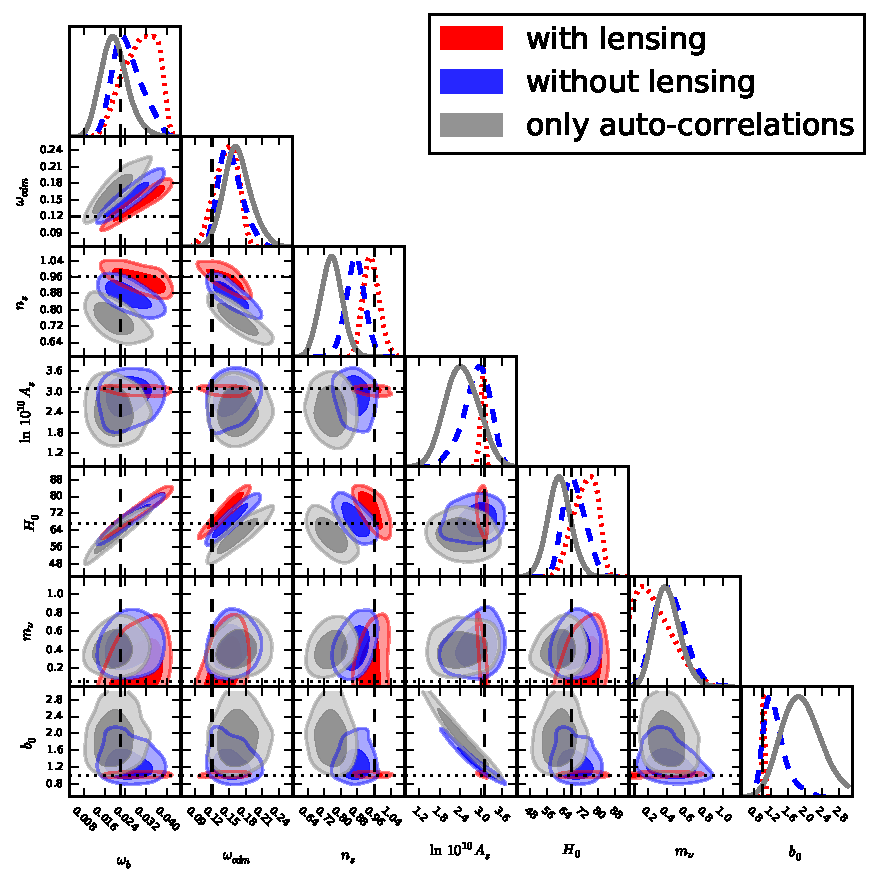
\includegraphics[scale=1]{figures/chapter-7/triangle_figure_MCDM_bias.pdf} 
\caption{Two- and 1-D posteriors for the cosmological parameters inferred from the full analysis including lensing (red dotted), an analysis neglecting lensing (blue dashed) and considering only auto-correlations (gray solid).
{The $68\%$ and $95\%$ confidence intervals are shown.}
Intersections between vertical and horizontal lines denote the fiducial cosmology.
}
\label{Fig:mcmc-flat-prior}
\end{figure}

\commentr{triangle plot and table. Discuss degeneracies, bias, current limits in neutrino mass, and show spectra for best fits}

\subsection{Gaussian prior}

\commentr{triangle plot and table. Conclusions change w.r.t to flat priors ?}

\begin{table}[!t]
\centering
\begin{tabular}{@{}cccccc}
\hline
\multicolumn{6}{c}{i) Consistently including lensing: $\Delta \chi^2 = 768.443$} \\
\hline
Parameter & Mean & best fit & $\sigma$ &\hspace{-0.52cm} shift: mean & best-fit \\
\hline
$\omega_b$ & $0.02225$ & $0.02225 $ &$0.00016 $ &  \quad$<0.1\sigma$ & $ <0.1\sigma$ \\
$\omega_{cdm}$ & $0.1202 $ & $0.1203 $ & \quad$0.0013 $ &  \quad$0.3\sigma$ & $0.4\sigma$ \\
$n_s$      & $0.9652 $ & $0.9636 $ & $0.0044 $ &  \quad$0.2\sigma$ & $ 0.2\sigma$ \\
$\ln10^{10}A_s$ & $3.090 $ & $3.092$ & $0.045 $ &  \quad$0.1\sigma$ & $ <0.1\sigma$ \\
$H_0\left[\frac{\text{km}}{\text{s}\cdot\text{Mpc}}\right]$      & $67.09$ & $67.16$ & $0.82$ &  \quad$0.2\sigma$ & $ 0.1\sigma$ \\
$m_{\nu}$\,[eV]  & $0.09$ & $0.08$ & $0.06$ & \quad $ 0.5\sigma$ & $ 0.3\sigma$ \\
$b_0$ & $1.006$ & $1.004$ & $0.026$ & $0.2\sigma$ & $0.2\sigma$ \\
\end{tabular}
\begin{tabular}{@{}cccccc}
\hline
\multicolumn{6}{c}{ii) Neglecting lensing: $\Delta \chi^2 = 2847.399$} \\
\hline
Parameter & Mean & best fit & $\sigma$ & \hspace{-0.52cm} shift: mean & best-fit \\
\hline
$\omega_b$ & $0.02221$ & $0.02221 $ & $0.00017 $ &  \quad$0.2\sigma$ & $0.2\sigma$ \\
$\omega_{cdm}$ & $0.1212$ & $0.1207$ & $0.0015$ &  \quad$1\sigma$ & $0.6\sigma$ \\
$n_s$      & $0.9638$ & $0.9637$ & $0.0049$ &  \quad$0.1\sigma$ & $0.2\sigma$ \\
$\ln10^{10}A_s$ & $ 2.368 $ & $2.446 $ & $ 0.428 $ &  \quad$1.7\sigma$ & $1.5\sigma$ \\
$H_0\left[\frac{\text{km}}{\text{s}\cdot\text{Mpc}}\right]$      & $65.83$ & $65.96$ & $0.92$ &  \quad$1.6\sigma$ & $1.4\sigma$ \\
$m_{\nu}$\,[eV]  & $0.35$ & $0.33$ & $0.06$ &  \quad$4.8\sigma$ & $4.5\sigma$ \\
$b_0$ & $1.574$ & $1.479$ & $0.339$ & $1.7\sigma$ & $1.4\sigma$\\
\end{tabular}
\begin{tabular}{@{}cccccc}
\hline
\multicolumn{6}{c}{\parbox[t]{4.4cm}{iii) Neglecting lensing: \\ \hspace*{0.9cm} (only auto-correlations)} $\Delta \chi^2 = 998.208$} \\
\hline
Parameter & Mean & best fit & $\sigma$ & \hspace{-0.52cm} shift: mean & best-fit\\
\hline
$\omega_b$ & $0.02219 $ & $0.02219 $ & $0.00017 $ &  \quad$0.3\sigma$ & $0.4\sigma$ \\
$\omega_{cdm}$ & $0.1222 $ & $0.1221 $ & $0.0014 $ &  \quad$1.7\sigma$ & $1.6\sigma$ \\
$n_s$      & $0.9640 $ & $0.9646 $ & $0.0050 $ &  \quad$0.1\sigma$ & $<0.1\sigma$ \\
$\ln10^{10}A_s$ & $1.672 $ & $1.488 $ & $0.427 $ &  \quad$3.3 \sigma$ & $3.8\sigma$ \\
$H_0\left[\frac{\text{km}}{\text{s}\cdot\text{Mpc}}\right]$      & $63.90 $ & $63.89$ & $0.98$ &  \quad$3.4 \sigma$ & $3.4\sigma$ \\
$m_{\nu}$\,[eV]  & $0.49$ & $0.49$ & $0.06$ &  \quad$7.1\sigma$ & $7\sigma$ \\
$b_0$ & $2.295$ & $2.461$ & $0.454$ & $2.9\sigma$ & $3.2\sigma$ \\
\end{tabular}

\caption{MCMC results (Gaussian prior). We show the mean and best fit values, the standard deviation and the amplitude of the shift of the mean and best-fit w.r.t the fiducial value in units of the standard deviation, $\sigma$, of the corresponding analysis. The large value of $\Delta \chi^2$ for case ii) shows that cross-correlations cannot be fitted if lensing is neglected.
}
\label{Table:mcmc-gaussian-prior}
\end{table}


\begin{figure}[bthp]
\centering
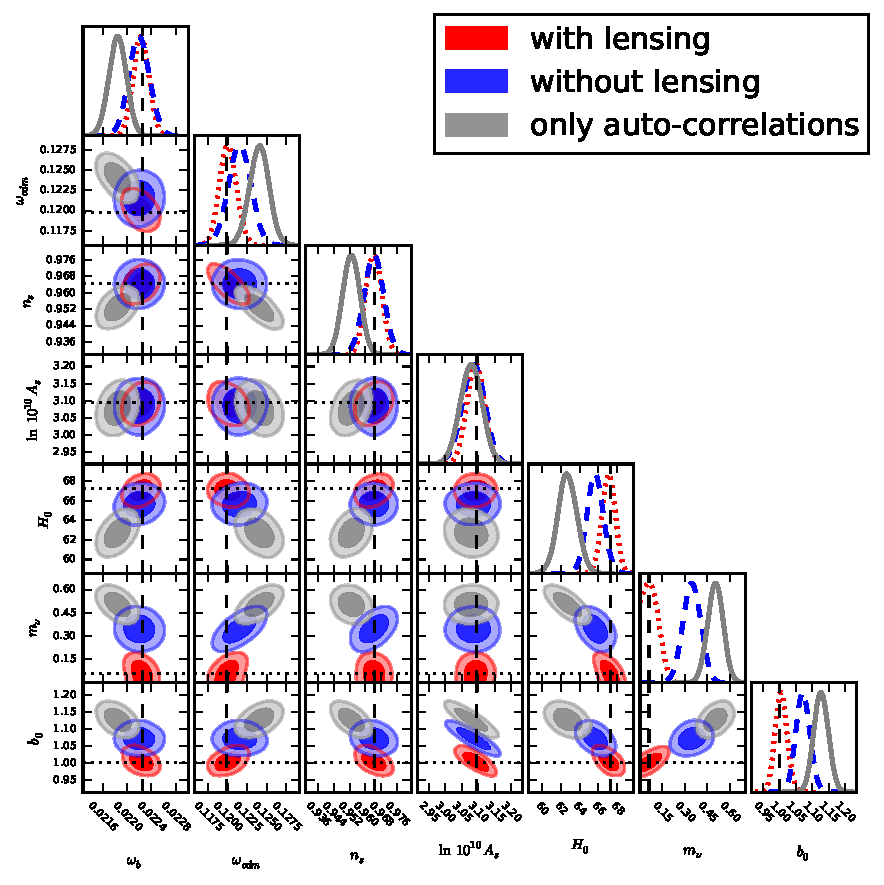
\includegraphics[scale=1]{figures/chapter-7/triangle_figure_MCDM_bias_cmb_prior.pdf}
\caption{Two- and 1-D posteriors for the cosmological parameters inferred from the full analysis including lensing (red dotted), an analysis neglecting lensing (blue dashed) and considering only auto-correlations (gray solid).
{The $68\%$ and $95\%$ confidence intervals are shown.}
Intersections between vertical and horizontal lines denote the fiducial cosmology.
}
\label{fig:mcmc-cmb-prior}
\end{figure}
\section{Conclusions}
\label{chapter:7:conclusions}

\commentr{lensing convergence must be included in galaxy clustering analysis. LSS breaks degeneracies.}

%The study of the large scale structure of the universe allows us to test the different cosmological models. The sky coverage and the deepness in redshift of  galaxy surveys have improved significantly in the past decades. This, in addition to the high precision CMB experiments, will able us to break the degeneracies in cosmological models that have plagued cosmology for quiet a while already. In particular, a better mapping of the matter distribution in the universe will help to put tighter constraints on the masses of neutrinos. Indeed, the clustering properties of the mass in the universe depend on the neutrino masses and possibly on their hierarchy. 

%Due to the experiments carried out in particle accelerators we know that neutrinos are massive. Nevertheless, we do not have a precise estimation for their masses which, in turn, unable us to estimate their total contribution to the energetic composition of the universe. Therefore, by measuring precisely the neutrino masses we can discriminate between different cosmological models since these predict distinct clustering properties. 

%In this chapter we do forecasts on the neutrino masses by using an Euclid-like survey. We use formalism of the angular power spectrum of the matter distribution and include the relevant relativistic effects, namely, lensing and redshift space distortions. The advantage of this formalism over the usual power spectrum $P(k;\, z=z_0)$ is that \dots \texttt{I must have a review of the literature and understand much better the two formalisms. A first advantage is related to the fact that the $C_{\ell}$ formalism deals with quantities which are directly observable without any model assumption. \\
%In the Euclid teleconference of Monday 14.12.2014 a Italian guy mentioned a third formalism. \\
%In particular, it would be important to understand why we include only the relativistic effects above. \\
%In addition, I must clarify the differences between spectroscopy and tomographic surveys. \\
%In connection with this last point, I should make clear what the power of Euclid will be.}

%In summary, in this chapter we aim to answer the following questions. First, will Euclid be able to measure the neutrino masses ?. Second, what error do we expect for such a survey ?. Third, will we be able to distinguish between different hierarchies with a Euclid-like survey ? 


\chapter{Testing isotropy and Gaussianity in the \textit{Planck} CMB estimates}
\label{chapter:8}

\section{Introduction} 

\texttt{This chapter is uncompleted. As can be seen in some of the figures shown below, the V-S-K method does not work properly when using masked maps: the oscillations in the spectra of V-S-K spectra do not come from the scanning of the sky, they are due to the masked region. The V-S-K method needs to be modified in order to include only unmasked regions because otherwise real cosmic features could be overlooked. We will try to extend this chapter, at least in two ways. First, we will implement the MASTER technique to deal only with unmasked regions of the sky. Second, in order to compare our results directly with those obtained by the Planck team, we must implement some of the component separation methods and use the same set of Gaussian isotropic simulations, that is, FFP6 and FFP8.}

The cosmological principle -- the assumption that the universe at sufficiently large scales is homogeneous and isotropic -- is one of the cornerstones of the standard model of cosmology (see, e.g., \cite{Robertson1935}; \cite{Walker1937}). Any significant indication of its violation would mean a serious caveat in our cosmological paradigm. Thus, to examine the validity of these assumptions is crucial. 

Recently, the \textit{Planck} collaboration has measured the anisotropies in the CMB with a much better precision than the \textit{Wilkinson Microwave Anisotropy Probe} (hereafter, \textit{WMAP}) (see, e.g., \cite{Spergel2003b}). According to the inflationary paradigm, at very early times the universe was filled with a hypothetical scalar field, the inflaton, whose fluctuations produced curvature perturbations distributed as a homogeneous and isotropic Gaussian random field. Cosmological perturbation theory establishes a relation between those primordial fluctuations and the CMB anisotropies, hence offering a unique probe to test models of the early universe. This relation implies that, in the framework of the cosmological principle, the CMB anisotropies are  statistically isotropic and Gaussian. Thus, testing the statistical properties of the CMB anisotropies allows us to examine  basic assumptions of the standard model of cosmology. In this work we will apply a statistical method different to those used by the \textit{Planck} team in \cite{PlanckXXIII} to look for possible deviations of Gaussianity and isotropy in the \textit{Planck} data.

The \textit{WMAP} team \cite{Spergel2003b} and other groups found some unexpected features -- anomalous properties in the CMB anisotropies which are statistically inconsistent with a best-fit $\Lambda$CDM model -- especially on large angular scales ($\ell < 600$); the list of anomalies includes lack of power on large angular scales \cite{Copi2007}, alignment of low-order multipoles (\cite{Tegmark2003}; \cite{Schwarz2004}; \cite{Bielewicz2005}; \cite{Land2005}), north-south asymmetry in both power spectra (\cite{Eriksen2004}; \cite{Hansen2009}) and several measures of non-Gaussianity (\cite{Eriksen2004a}; \cite{Eriksen2005}; \cite{Rath2007}; \cite{Rath2009}), the cold spot (\cite{Vielva2004}; \cite{Cruz2005}), and parity asymmetry in the power spectrum \cite{Kim2010a}. Not long ago, the \textit{Planck} team has confirmed the observation of those large scale anomalies. Bearing in mind that both \textit{Planck} and \textit{WMAP} are cosmic variance limited, the presence of those unexpected features in the \textit{WMAP} and \textit{Planck} data could be, in principle, due to unaccounted systematic errors, non-subtracted foreground contamination, or more interestingly, it could have a cosmological origin. On the one hand, the fact that two independent experiments have observed the same features reduces drastically the possibility that systematics errors be the source of these anomalies \cite{Larson2014}. On the other hand, unresolved foreground and the more appealing cosmological origin need to be studied further. 

In \cite{PlanckXXIII} the \textit{Plank} team has tested the Gaussianity and isotropy of  the CMB anisotropies and determined the statistical significance of their findings with a set of Gaussian, isotropic simulations of the CMB sky, namely, the ``Full Focal Plane'' (FFP6) simulations. They have used several statistical methods including the study of one-dimensional moments, N-point correlation functions, Minkowski functionals, wavelet, bispectrum and phase correlations. Several of those statistical methods (e.g., N-point correlation functions, the Minkowski functionals, and the bispectrum) show consistency with Gaussianity and isotropy regardless of the mask, the component separation and the resolution of the CMB maps used ($N_{side}$). Nevertheless, there is inconsistency with the FFP6 simulations when employing other methods. On the one hand, in their one-dimensional moments analysis they found that the variance is anomalously low at all considered resolutions ($N_{side}=2048,\, 512,\, 64,\, 32,\, 16$) and that the skewness (kurtosis) is anomalously low (high) at low resolutions ($N_{side}=64,\,32,\,16$). On the other hand, when using the wavelet statistics they also found inconsistencies. In particular, they report skewness (kurtosis) at small (intermediate) scales significantly lower (greater) than in the simulations. Finally, the most important discrepancy between data and simulations appears when analysing the data with the method of surrogates. The \textit{Planck} team found presence of pronounced anisotropy and also correlations between the low-$\ell$ Fourier phases in the analysed CMB maps, findings which turn out to be robust regardless of reference frame and component separation method. Similar results were obtained previously in \textit{WMAP} data \cite{Rath2009}. 

It is of great importance for the standard model of cosmology to clarify those discrepancies between the isotropic, Gaussian simulations and the \textit{Planck} data. In this paper we will test isotropy and Gaussianity by employing a blind analysis which has been applied in previous works to \textit{WMAP} data and assess the statistical significance of our results by using a set of Gaussian, isotropic simulations of the CMB sky. The method (hereafter, V-S-K method) consists of a set of statistical estimators which measure variance, skewness, and kurtosis in patches of the sky. The V-S-K method is similar to the wavelet statistics employed by the \textit{Planck} collaboration but, since our analysis works in real space, it localizes possible non-subtracted foregrounds and may provide the angular scale of possible deviations of Gaussianity and isotropy in the CMB anisotropies. Recently, the V-S-K method was used in \cite{Bernui2014} and in \cite{Bernui2014a} to study the north-south asymmetry phenomenon and non-Gaussianity in CMB anisotropies, respectively. However, the authors used overlapping patches of the sky when defining their estimators, possibly introducing spurious correlations in their estimations. Moreover, they did not use CMB maps in the full \textit{Planck} resolution ($N_{side}=2048$); even though this reduces the noise in the data (dominant at small scales), it also increases the error in the estimations. Since the V-S-K method is built to test large scales, the latter would not be crucial, but it would mean an important reduction in the statistical significance of the results.

In the present chapter, we start out giving a brief description of the data (Section \ref{s:data}) and then present the V-S-K method for non-overlapping patches of the sky (Section \ref{s:method}). The V-S-K method is subsequently applied to both \textit{Planck} data and Gaussian, isotropic simulations of the CMB sky and our results are discussed in Section \ref{s:results}. We conclude in Section \ref{s:summary}.

\section{Data}
\label{s:data}

In this work we make use of part of the \textit{Planck}-2013 data release corresponding to the nominal period of the \textit{Planck} mission. We utilise some of the available masks, the two available inpainted CMB maps, and the nearly full-sky foreground cleaned CMB maps resulting from four  component separation algorithms applied by the \textit{Planck} team \cite{Ade2014d}, viz., \texttt{Commander-Ruler, NILC, SEVEM} and \texttt{SMICA}. The maps and masks were provided in \textsc{HEALPix}\footnote{http://healpix.sourceforge.net} format, with a pixel size defined by the $N_{side}$ parameter. 

Throughout the paper we use the standardized common mask U73 (sky coverage $f_{sky} = 73$ per cent). However, when studying the mask dependence of our analysis we use the confidence mask VALMASK ($f_{sky} = 89$ per cent) and the mask of the inpainted regions INP$\_$MASK ($f_{sky} = 97$ per cent) of the \texttt{SMICA} CMB estimate. Where appropriate, we have changed the resolution of the mask and maps, originally having $N_{side}=2048$. In particular, we have degraded the data to have $N_{side}=1024,\, 512$, and $256$. When degrading the mask we have followed the same conservative approach used by the \textit{Planck} team: after degrading the mask to the final resolution using the \textsc{ud$\_$grade HEALPix} routine, any pixel having a value lower than $0.8$ has been set to zero. 

Finally, in order to assess the significance of any anisotropic or non-Gaussian signal in the data, we resort to a set of $2000$ simulated Gaussian, isotropic CMB maps. The Monte Carlo simulations were generated using the \textsc{synfast HEALPix} routine based on the \textit{Planck} best-fit power spectrum and having an effective Gaussian beam $\texttt{FWHM}=5$ arcmin.

\section{V-S-K Method}
\label{s:method}

The method, which in the scope of this study will be referred to as V-S-K method, was first introduced and applied to \textit{WMAP} data in \cite{Bernui2009}  (see also \cite{Bernui2010,Bernui2012}). However, as originally proposed, the method uses overlapping patches in the sky that, as mentioned earlier, might introduce spurious correlations in the data. The V-S-K method was modified to employ non-overlapping patches of the sky and applied to \textit{WMAP} data in \cite{Cardona2012} and simulations in \cite{Cardona2013}. Given a full-sky CMB map in \textsc{HEALPix} format with parameter $N_{side}$, the construction of the estimators in the V-S-K method proceeds as follows. 

\begin{enumerate}
\item We superimpose on the original CMB map a \textsc{HEALPix} grid with much lower resolution $N'_{side}$ than that of the CMB map (e.g., $N'_{side} = 2,4,8,\dots$). Thus, we have a set of $12 \times N^{'2}_{side}$ non-overlapping patches in the sky, each patch having equal number $N_p$ of pixels belonging to the initial CMB map\footnote{For a full-sky CMB map with parameter $N_{side}$ the number of pixels is given by $12 \times N^2_{side}$. Then, the number of pixels per patch is given by $\left(N_{side}/N'_{side}\right)^2$.}. %Hereafter, we will call each one of those non-overlapping patches cells.
\item For each patch we compute sample variance,
\begin{equation}
\label{eq:1}
V_j = \frac{1}{N_p -1} \sum_{i=1}^{N_p} (T_i - \bar{T})^2 = \frac{N_p}{N_p -1} \sigma_j^2 ,
\end{equation}
sample skewness,
\begin{equation}
\label{eq:2}
S_j = \frac{1}{N_p \sigma_j^3} \sum_{i=1}^{N_p} (T_i - \bar{T})^3 ,
\end{equation}
and sample kurtosis,
\begin{equation}
\label{eq:3}
K_j = \frac{1}{N_p \sigma_j^4} \sum_{i=1}^{N_p} (T_i - \bar{T})^4 - 3 ,
\end{equation}
where $j$ numbers the non-overlapping patches, $T_i$ is the temperature at the $i^{th}$ pixel in the $j^{th}$ patch, $\bar{T}$ is the CMB mean temperature in the $j^{th}$ patch, and $\sigma_j$ denotes the standard deviation of the CMB data in the $j^{th}$ patch. We compute sample variance, sample skewness, and sample kurtosis including only unmasked pixels; any patch for which more than $20$ per cent of the area is masked is set to zero.
\item The result of computing $V_j$, $S_j$, and $K_j$ for all the patches is three different maps, namely, one map of sample variance, one map of sample skewness and one map of sample kurtosis. Henceforward, we will refer to those maps as V-map, S-map and K-map, respectively.
\item Since the V-map, S-map, and the K-map are signals on the sphere, they can be written in terms of a spectral representation. For instance, for the V-map we have 
\begin{equation}
\label{eq:4}
V(\mathbf{x}) = \sum^{\infty}_{\ell=0} \sum^{\ell}_{m=-\ell} v_{\ell m} Y_{\ell m} (\mathbf{x})
\end{equation}

\noindent where $\mathbf{x}$ is a unit direction vector, $Y_{\ell m}$ the spherical harmonics and 

\begin{equation}
v_{\ell m} = \int d\mathbf{x} V(\mathbf{x}) Y^*_{\ell m}(\mathbf{x}),
\end{equation}

\noindent $m=0,\pm1,\dots,\pm \ell$, $\ell=0,1,2,\dots$. Similar expressions are satisfied by S-map and K-map. 

\item Finally, we perform the harmonic analysis of the V-map, S-map, and K-map with the help of the \textsc{anafast HEALPix} routine with maximum spherical harmonic order given by $\ell_{max}=3\times N'_{side}-1$. Taking as an example the $V(\mathbf{x})$ signal again, we have 
\begin{equation}
\label{eq:5}
V_\ell = \frac{1}{2 \ell +1} \sum_{m} |v_{\ell m}|^2 ,
\end{equation}
where $V_{\ell}$ is the angular power spectrum of the V-map. Similar expressions  $S_\ell$ and $K_\ell$ apply for S-map and K-map, respectively.
\end{enumerate}

Throughout this paper we quantify the degree of agreement between the Gaussian, isotropic simulations and the observations by a simple $\chi^2$ test which has been performed separately for the V, S, and K estimators. For instance, for the V estimator we define $\chi^2_{V}$ as 

\begin{equation}
\chi^2_{V} = \sum_{\ell \ell'} \left( V_\ell - \left\langle V_\ell \right\rangle_G \right) C^{-1}_{\ell \ell'} \left( V_{\ell'} - \left\langle V_{\ell'} \right\rangle_G\right),
\label{eq:6}
\end{equation}

with analogous expressions for S and K estimators. In equation (\ref{eq:6}) $V_\ell$ is the angular power spectrum of a V-map computed out of a given full-sky CMB map, $\left\langle V_\ell \right\rangle_G$ the corresponding average from a set of Gaussian, isotropic simulations, and 

\begin{equation}
C_{\ell \ell'} = \left\langle \left( V_\ell - \left\langle V_\ell \right\rangle_G \right) \left( V_{\ell'} - \left\langle V_{\ell'} \right\rangle_G \right)\right\rangle_G
\end{equation}

the covariance matrix from a different set of Gaussian, isotropic simulations.

\section{Results}
\label{s:results}

We now apply the V-S-K method to \textit{Planck} data. We start by examining how the method works when using full-sky ($f_{sky}=100$ per cent) CMB maps. In particular, we use the two inpainted CMB estimates released by the \textit{Planck} collaboration, namely, the $N_{side}=2048$ inpainted \texttt{SMICA} and \texttt{NILC}. 

In Fig. \ref{Fig:1} we show angular power spectra for the V-map, S-map, and the K-map computed for those CMB estimates and for $1000$ Gaussian, isotropic simulations using $N'_{side} = 4$. As expected, the mean angular power spectra for the simulations do not exhibit scale dependence. The angular power spectrum of the variance maps, $V_{\ell}$, for the two considered CMB estimates show  departure from the null hypothesis. In particular, inpainted \texttt{SMICA} has both a dipole and a quadrupole outside the $95$ per cent confidence region. This dipolar structure,  the so-called north-south asymmetry, was also found in \textit{WMAP} and \textit{Planck} data (\cite{Eriksen2004}; \cite{Hansen2009}; \cite{PlanckXXIII}; \cite{Akrami2014a}). Using different values of the parameter $N'_{side}$, we verified the robustness of this result. The angular power spectra of the corresponding S-maps, $S_{\ell}$, is consistent with the null hypothesis. Although at multipoles $\ell \geq 10$ the inpainted \texttt{NILC} shows  a little tension with regard to the simulations, we could verify that this mismatch vanishes when $N'_{side}$ increases. The most remarkable difference between the two CMB estimates is brought out when looking at the corresponding $K_{\ell}$. The inpainting technique applied to the \texttt{NILC} CMB estimate seems to induce kurtosis at all considered scales. This contribution, however, diminishes for increasing $N'_{side}$. The same applies for the multipole $\ell=5$ in the inpainted \texttt{SMICA}. In Fig. \ref{Fig:2} we show the $\chi^2$ analysis for the spectra in Fig. \ref{Fig:1}. Note that due to this discrepancy we do not show the $\chi^2$ value for the inpainted \texttt{NILC} $K_{\ell}$. In Table \ref{table:1} we show the lower-tail probability computed out of N-pdf $\chi^2$ for different values of the parameter $N'_{side}$. The V estimator gives consistent results for the two CMB estimates and does not seem to strongly depend on the $N'_{side}$ parameter. The probabilities are high for all the $N'_{side}$ considered. The probabilities for the S estimator vary consistently with $N'_{side}$. However, for $N'_{side}=4$ the probability is high in the inpainted \texttt{NILC}. The probabilities for the K estimator increase with $N'_{side}$ for inpainted \texttt{SMICA} and remain constant for inpainted \texttt{NILC} because of the discrepancy shown we discussed previously.

\begin{figure}
\centering
%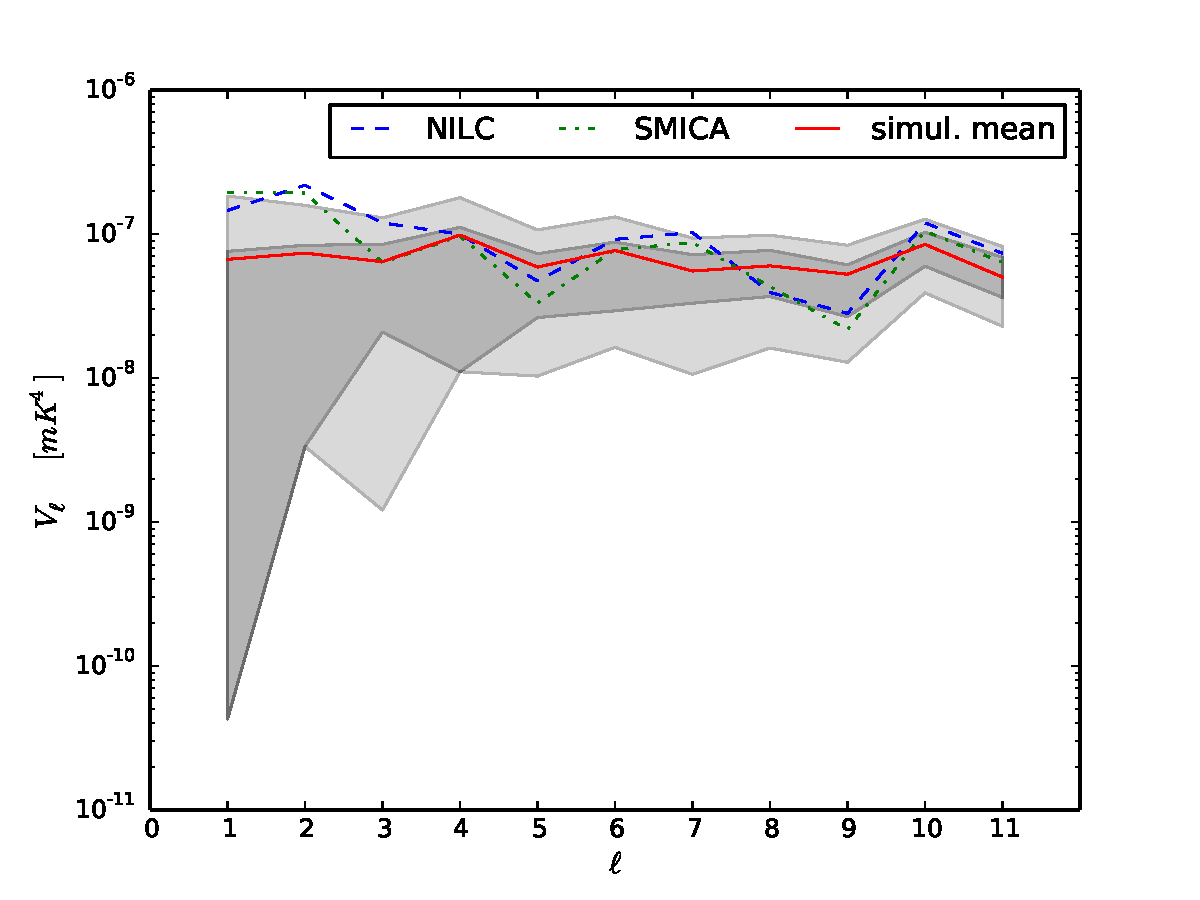
\includegraphics[scale=0.45]{Inp_Vl.pdf}\\
%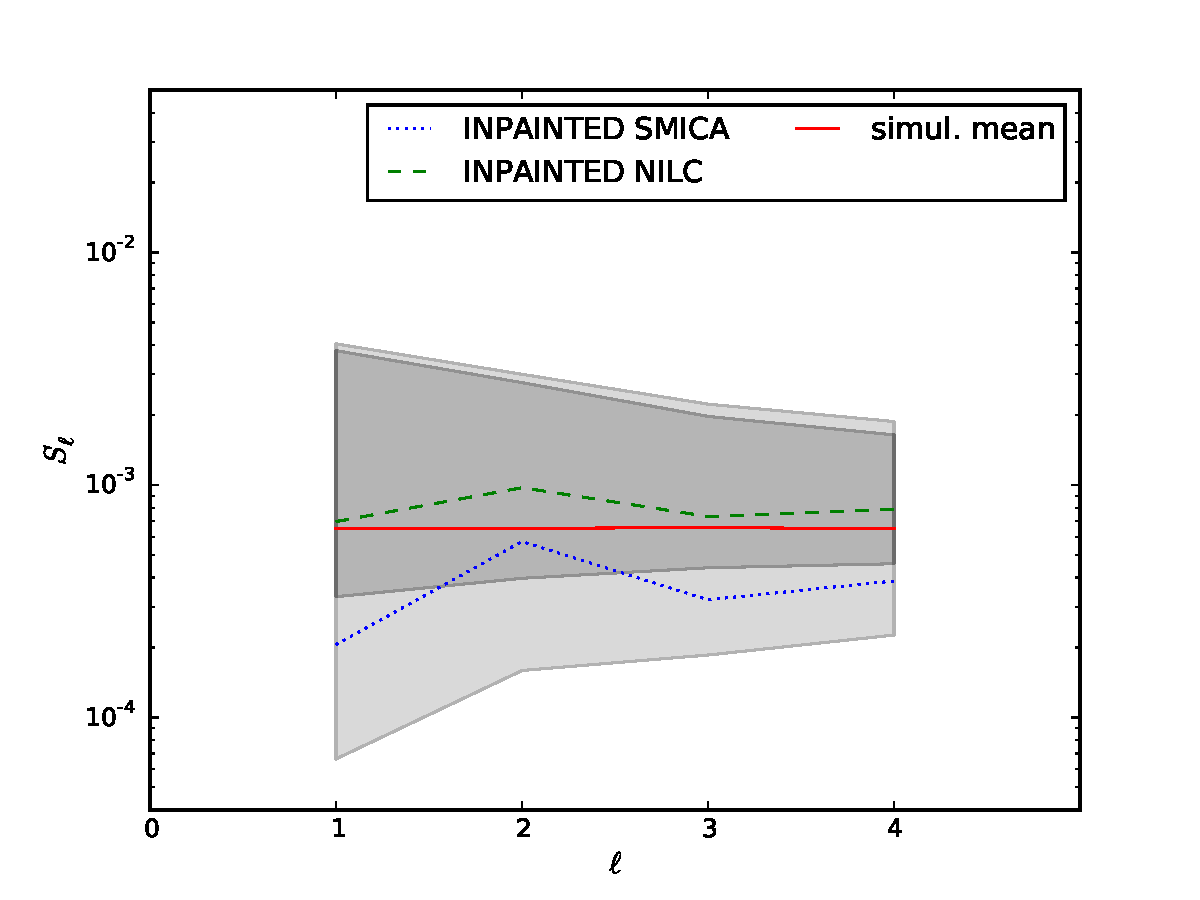
\includegraphics[scale=0.45]{Inp_Sl.pdf}\\
%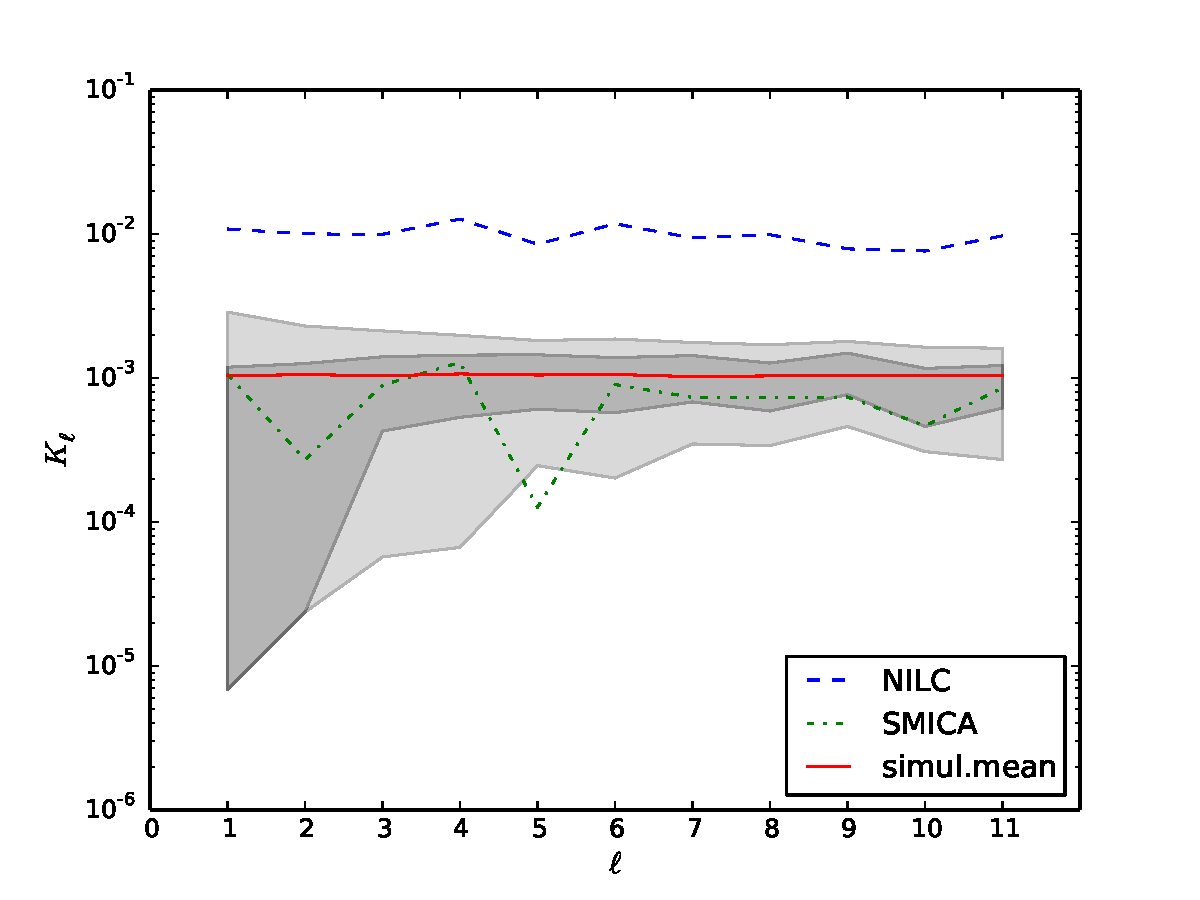
\includegraphics[scale=0.45]{Inp_Kl.pdf}
\caption{Angular power spectra for the $N'_{side} = 4$ V-map, S-map, and K-map computed out of the full-sky $N_{side} = 2048$ inpainted CMB estimates. The red solid line indicates the mean for $1000$ Monte Carlo simulations and the shaded dark and light gray regions indicate the $68$ per cent and $95$ per cent confidence regions, respectively.}
\label{Fig:1}
\end{figure}

\begin{figure}
\centering
%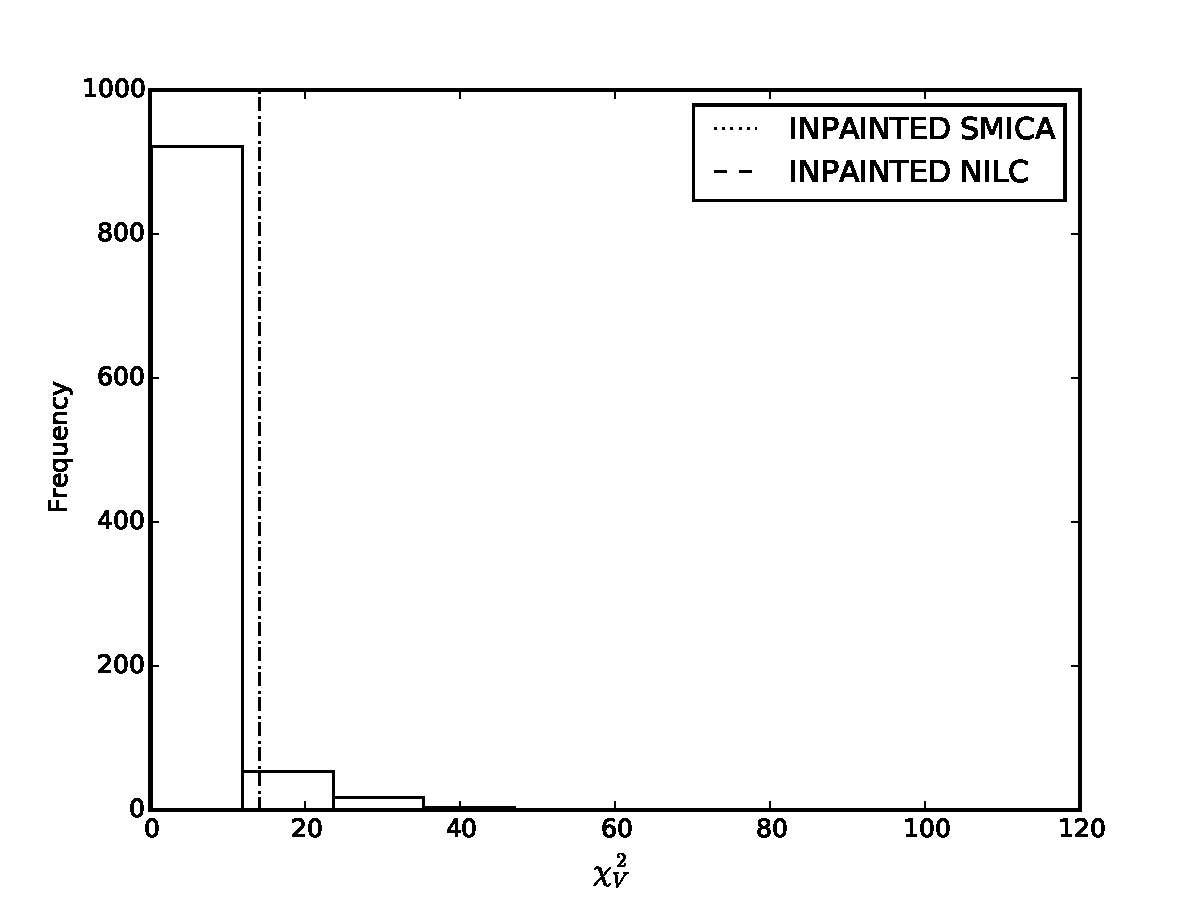
\includegraphics[scale=0.45]{vchi2.pdf}\\
%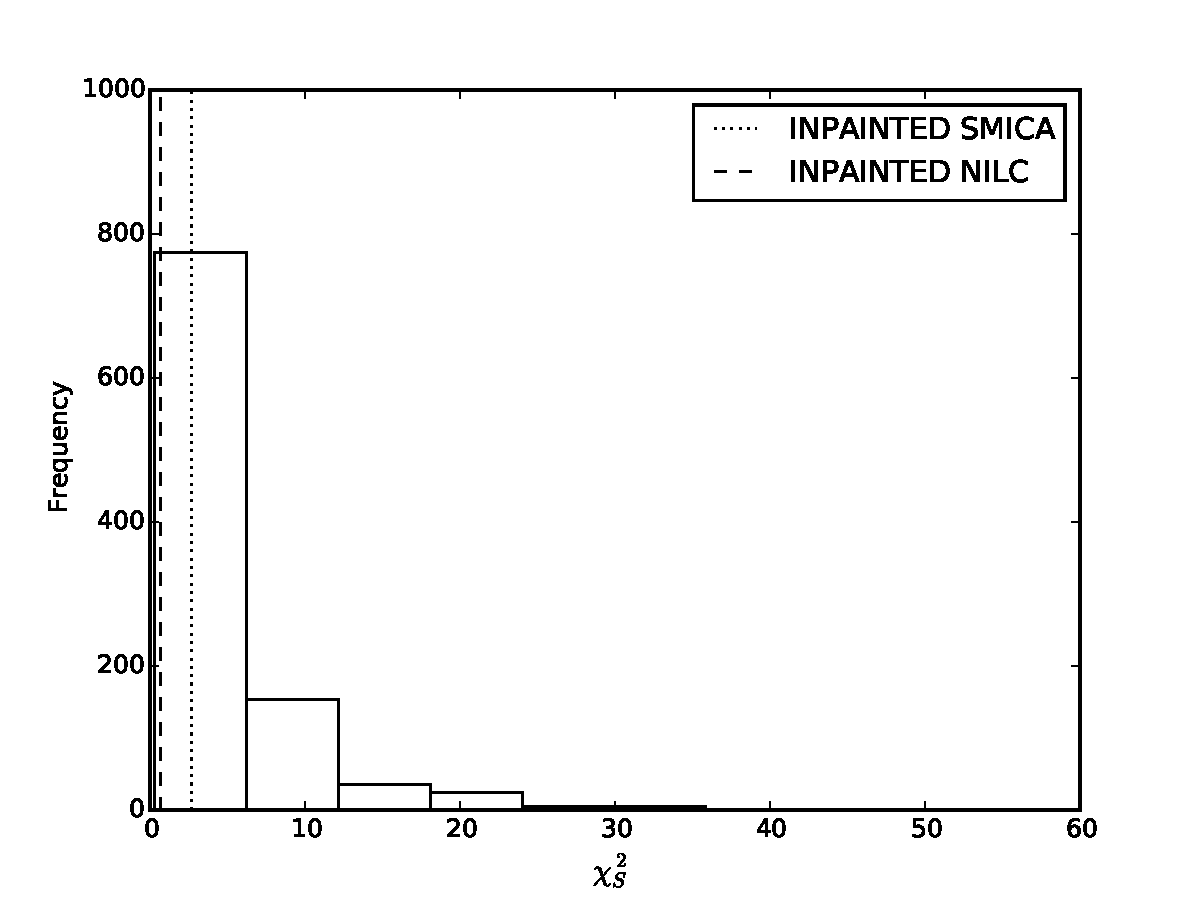
\includegraphics[scale=0.45]{schi2.pdf}\\
%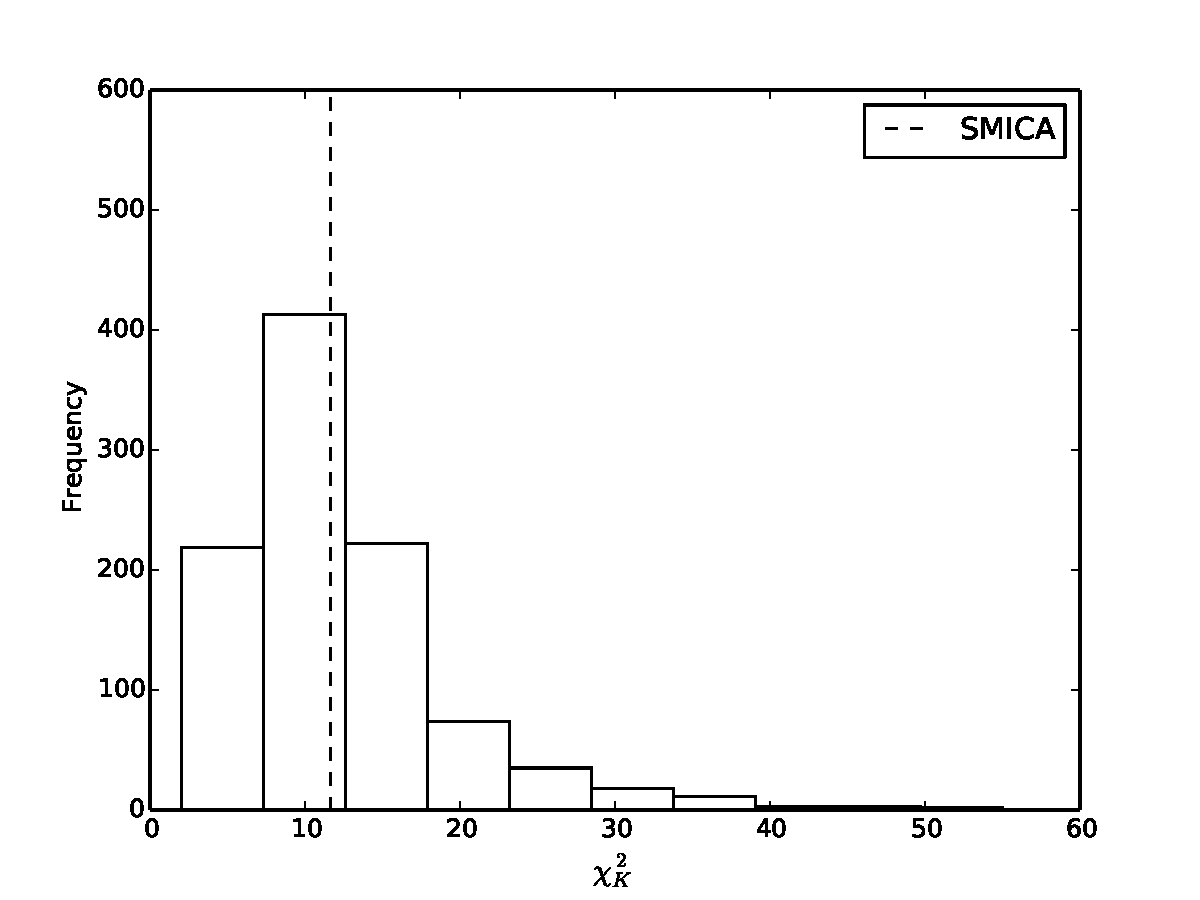
\includegraphics[scale=0.45]{kchi2.pdf}
\caption{N-pdf $\chi^ 2$ for the angular power spectra shown in Fig. \ref{Fig:1}. The vertical lines show values for the corresponding CMB estimates.}
\label{Fig:2}
\end{figure}

\begin{table}
\centering
\caption{Lower-tail probability for the V, S, K estimators at different resolutions, for the $N_{side} = 2048$ inpainted \texttt{SMICA} and \texttt{NILC}.}
\label{table:1}
\begin{tabular}{@{}lcccc}
\hline 
  & & Probability & \\
\hline  
CMB estimate & V & S & K \\ 
\hline  
 & & $N'_{side}=2$ & \\
\texttt{SMICA} & $0.977$ & $0.355$ & $0.038$ \\ 
\texttt{NILC} & $0.972$ & $0.781$ & $1.0$  \\
 & & $ N'_{side} = 4 $ & \\
\texttt{SMICA} & $0.998$ & $0.718$ & $0.585$ \\
\texttt{NILC} & $0.985$ & $0.988$ & $1.0$ \\
 & & $N'_{side} = 8$ & \\
 \texttt{SMICA} & $1.0$ & $0.374$ & $0.745$ \\
 \texttt{NILC} & $0.995$ & $0.385$ & $1.0$ \\
 & & $N'_{side} = 16$ & \\
 \texttt{SMICA} & $1.0$ & $0.241$ & $0.786$ \\
 \texttt{NILC} & $1.0$ & $0.093$ & $1.0$ \\
\end{tabular} 
\end{table}

According to the previous analysis the inpainting technique applied to \texttt{NILC} might induce some deviations of the null hypothesis. Therefore we now apply the V-S-K method to the almost full-sky $N_{side}=2048$ CMB estimates. We examine the four component separation methods mentioned above and use the U73 mask. In Fig. \ref{Fig:3} we illustrate, as an example, the V-map, S-map, and the K-map for the \texttt{SMICA} estimate. In Fig. \ref{Fig:4} we plot the corresponding angular power spectra $V_{\ell},\, S_{\ell},\, $ and $K_{\ell}$ computed for the four component separation CMB estimates. As can be seen, all the four estimates seem to be consistent with the null hypothesis. Nevertheless, note that due to the masked regions in the V-maps, S-maps, and K-maps the angular power spectra of the simulations are not any longer scale independent, the effect being much more visible in the case of $V_{\ell}$ because of the much more different value associated with the masked pixels. A possible modification in the method to include only unmasked regions in the computation of the angular power spectrum would be necessary to avoid these spurious features. Nevertheless, since in this work we want to test whether or not the \textit{Planck} data are consistent with the null hypothesis, we will not include  this modification in the present paper. Such a modification would require to adapt the V-S-K method as explained in \cite{Gorski1994} and \cite{Hivon2002}.

Comparing the results of the full-sky inpainted CMB maps with those of the almost full-sky CMB maps, we can see that there is no departure from the null hypothesis in the NILC CMB estimate when the inpainted regions are disregarded. Thus, the discrepancy observed in the full-sky map for the K estimator seems to be caused by the inpainted regions in the inpainted \texttt{NILC}. The four component separation methods exhibit a dipole in the V-maps outside the $95$ per cent confidence region for $N'_{side}=2$, but this feature disappears gradually  when increasing the parameter $N'_{side}$. This might be due to the fact that by construction the method V-S-K, as we have applied it here, disregards patches (patches set to zero) with less than $80$ per cent of unmasked pixels and therefore it is not guaranteed that the sky fraction (fraction of the sky having patches with non zero value) be the same for each $N'_{side}$. 

Since all the four component separation methods give pretty similar results and to avoid circumlocution, in Table \ref{table:2} we present the lower-tail probabilities only for the \texttt{SMICA} CMB estimate. We have examined the dependence of our results on the parameters $N_{side}$ and $N'_{side}$. In summary, we do not see significant deviation of the null hypothesis for almost all the possible combinations of parameters considered, with the exception of the V estimator for $N_{side}=2048$ and $N'_{side}=8,\,16$ where there is a discrepancy with the simulations.
 

\begin{figure}
\centering
%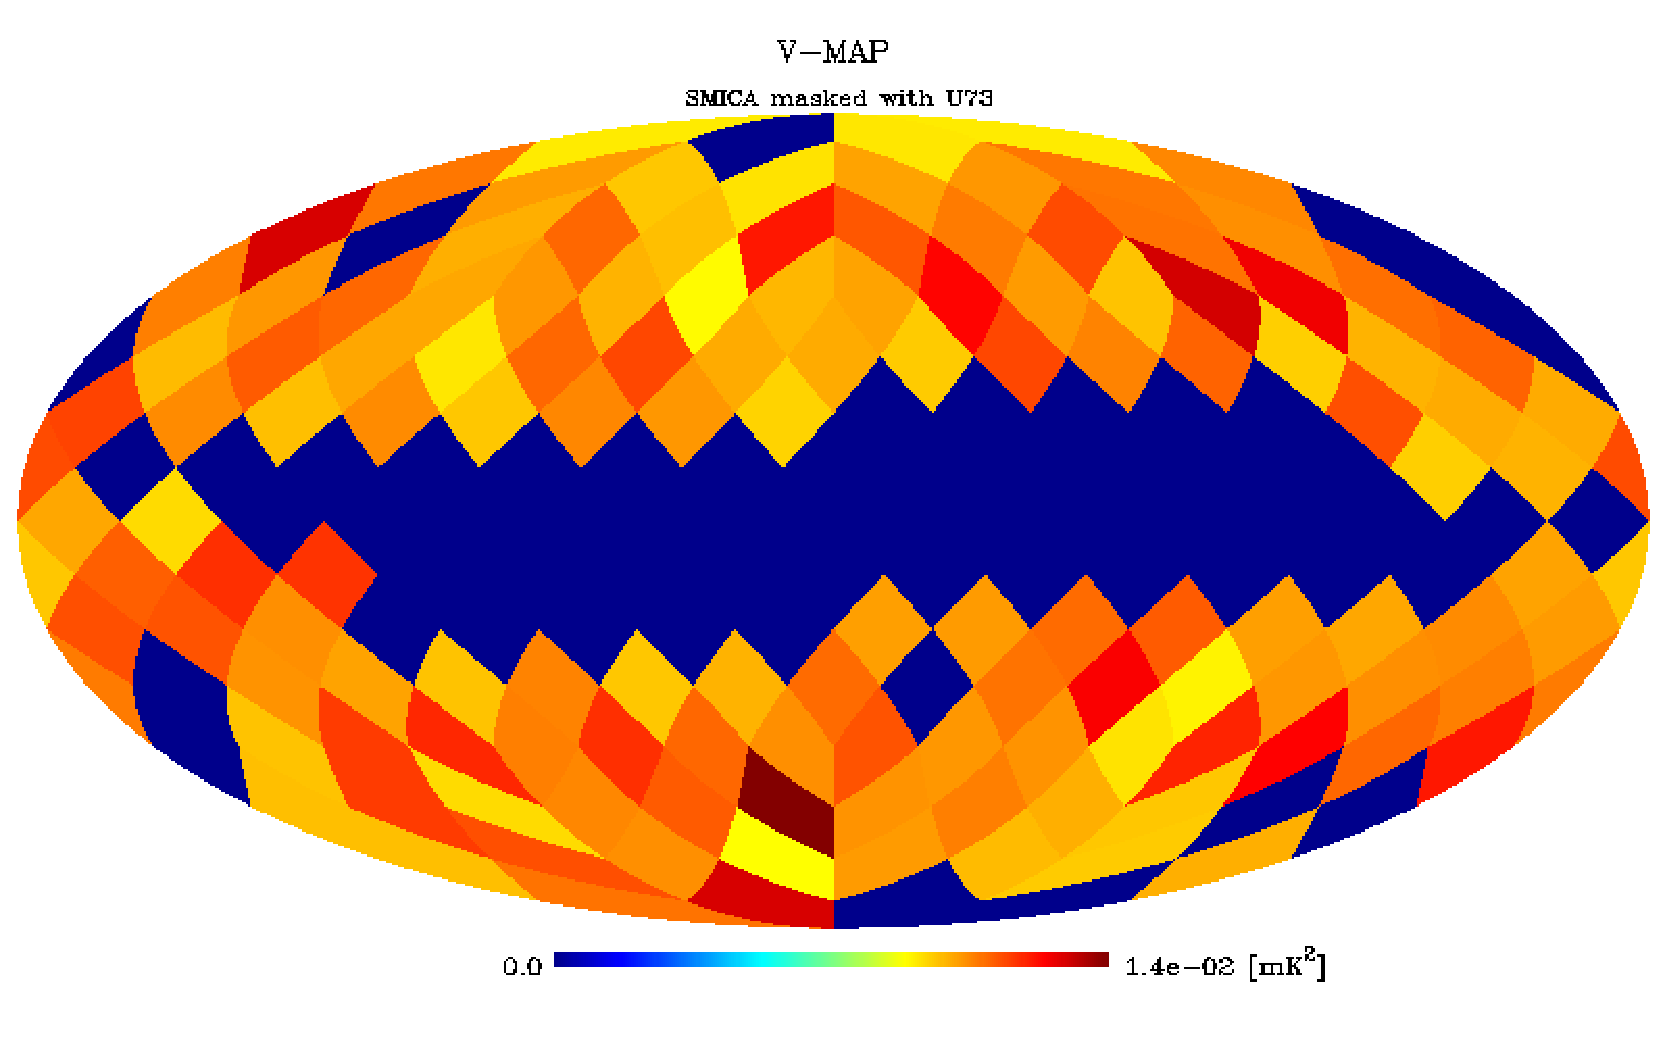
\includegraphics[scale=0.3]{vmap.pdf}\\
%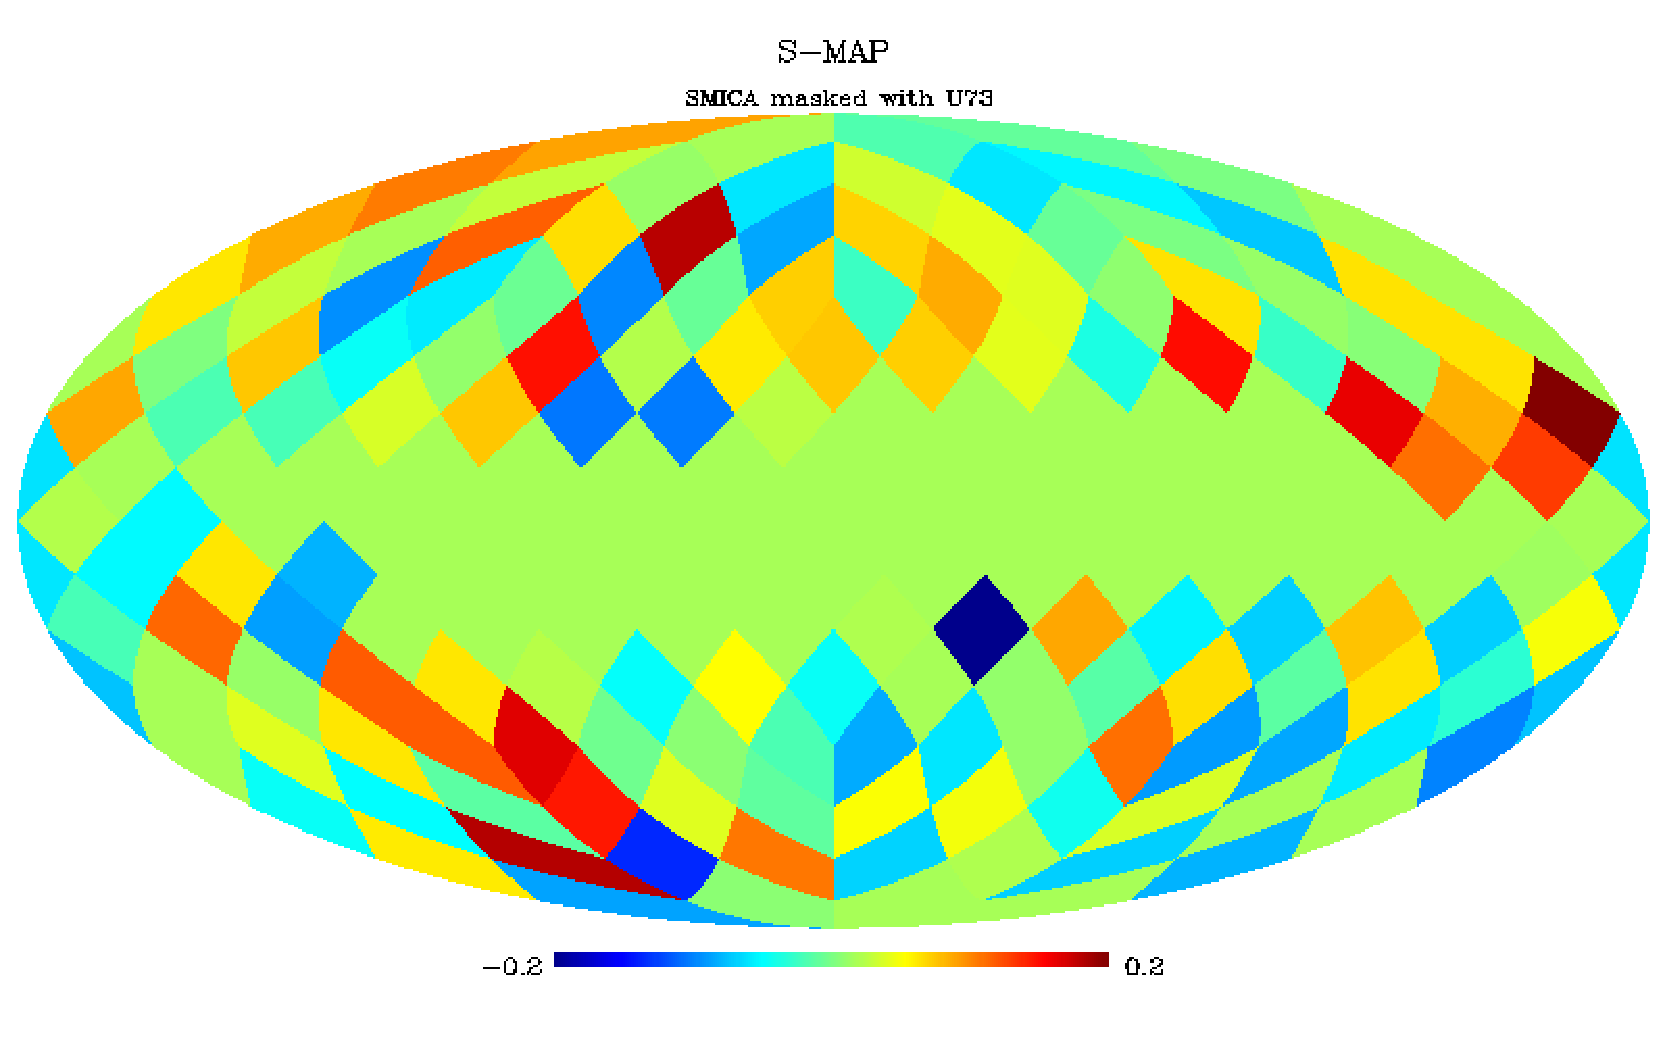
\includegraphics[scale=0.3]{smap.pdf}\\
%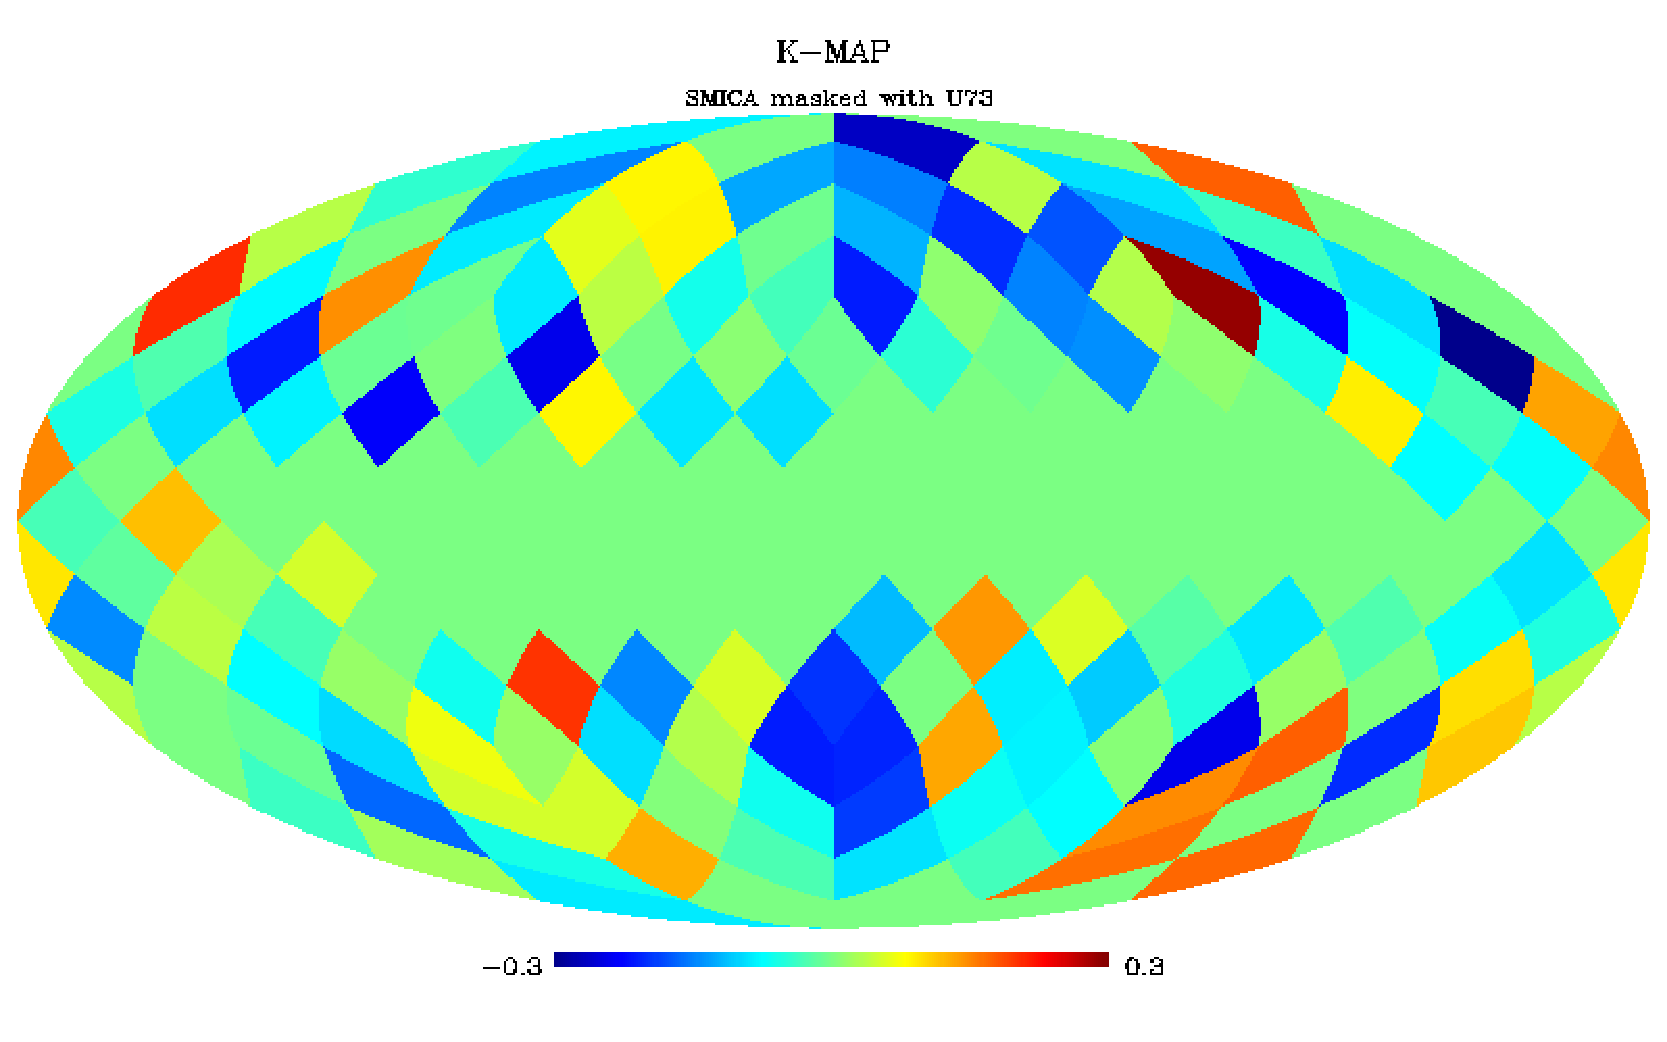
\includegraphics[scale=0.3]{kmap.pdf}
\caption{$N'_{side = 4}$ V-map (\textit{upper}), S-map (\textit{middle}), and K-map (\textit{lower}) for the $N_{side} = 2048$ SMICA CMB estimate masked with the U73 mask.}
\label{Fig:3}
\end{figure}

\begin{figure}
\centering
%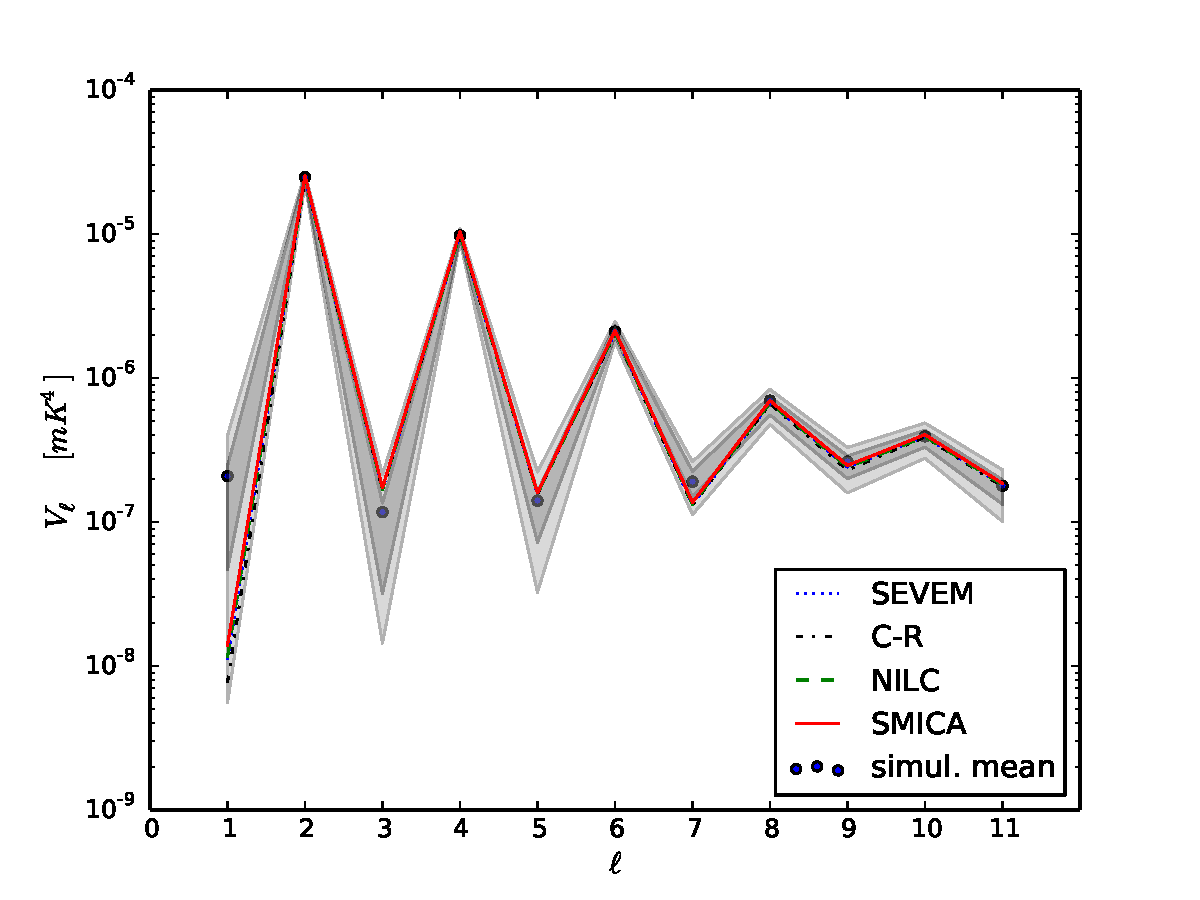
\includegraphics[scale=0.45]{Vl_u73.pdf}\\
%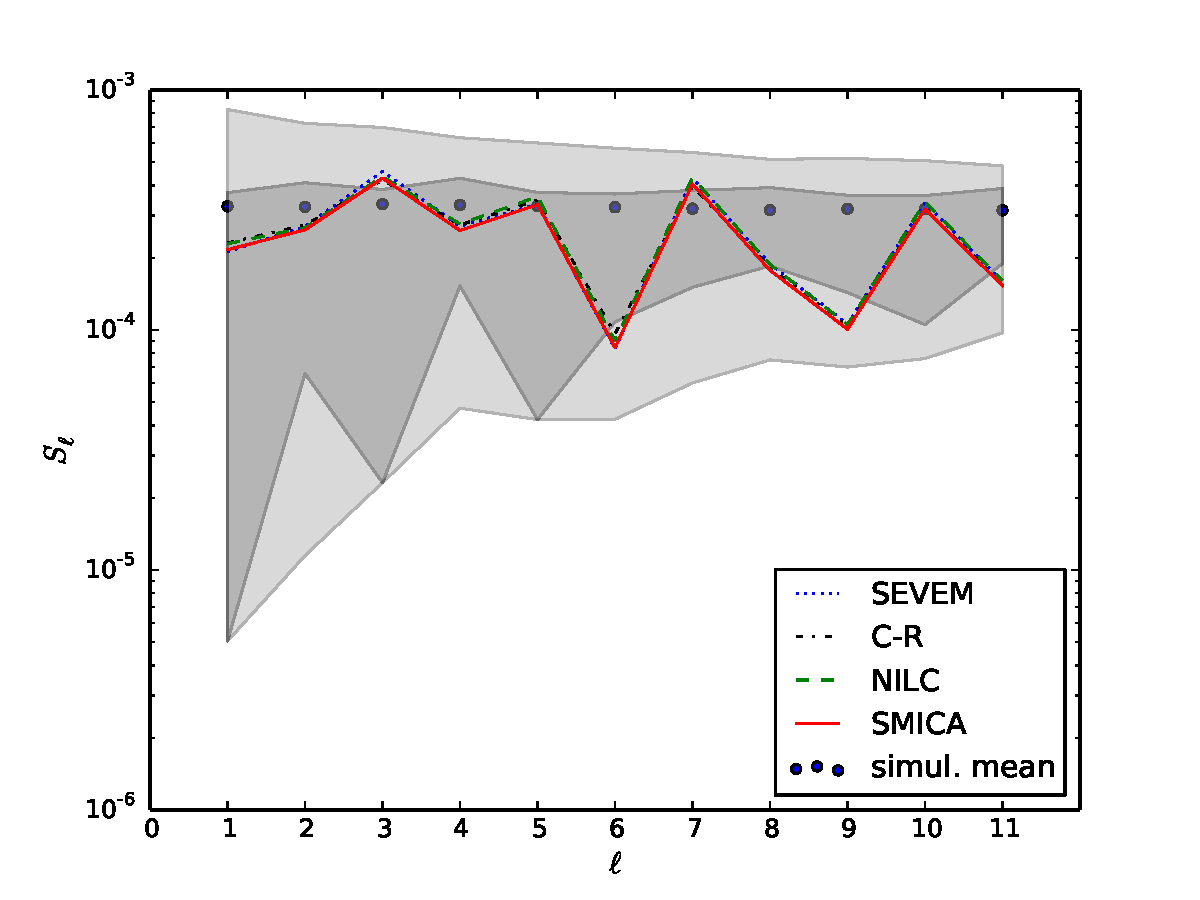
\includegraphics[scale=0.45]{Sl_u73.pdf}\\
%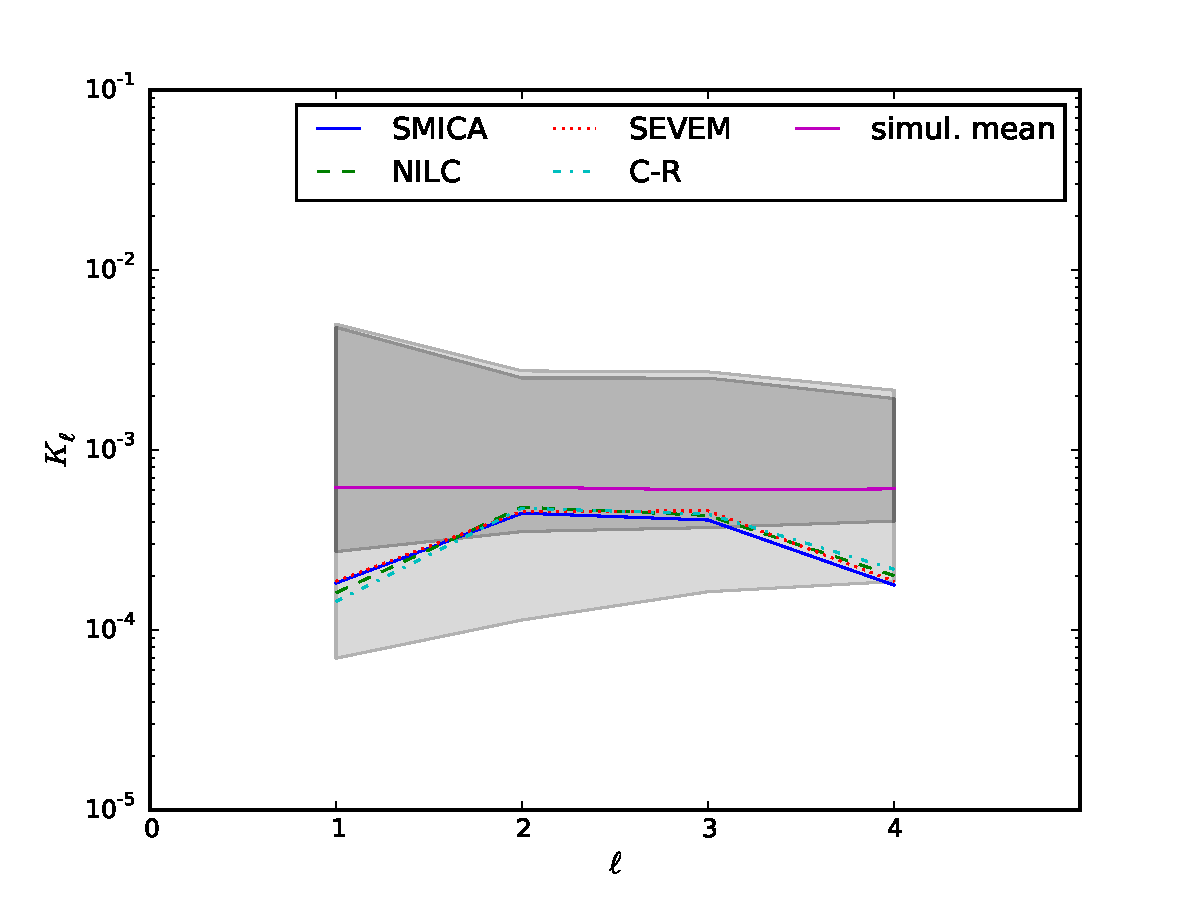
\includegraphics[scale=0.45]{Kl_u73.pdf}
\caption{Angular power spectra of the $N'_{side} = 4$ V-map, S-map, and K-map for the four $N_{side} = 2048$ CMB estimates. The blue dots indicate the mean angular power spectrum for $1000$ Monte Carlo simulations and the shaded dark and light gray regions indicate the $68$ per cent and $95$ per cent confidence regions, respectively.}
\label{Fig:4}
\end{figure}

We have also studied the mask dependence of the V-S-K method. The results for both the confidence mask and the mask of inpainted regions for \texttt{SMICA} are shown in Table \ref{table:3}. In order to facilitate the comparison some of the results for the mask U73 are repeated. The sky coverage of the considered masks does not seem to affect the results considerably in any of the estimators. 

\begin{table}
\centering
\caption{Lower-tail probability for the V, S, K estimators at different resolutions $N'_{side}$, for different resolutions $N_{side}$ of the  \texttt{SMICA} CMB estimate using the U73 mask.}
\label{table:2}
\begin{tabular}{@{}lcccc}
\hline 
  & & Probability & \\
\hline  
$N'_{side}$ & V & S & K \\ 
\hline  
 & & $N_{side}=2048$ & \\
$2$ & $0.929 $ & $ 0.152$ & $0.513 $ \\ 
$4$ & $ 0.754$ & $0.656 $ & $0.292 $  \\
$8$ & $ 1.0$ & $ 0.094 $ & $ 0.412 $  \\
$16$ & $ 1.0 $ & $ 0.391 $ & $ 0.439 $  \\
 & & $ N_{side} = 1024 $ & \\
$2$ & $ 0.869 $ & $ 0.151 $ & $ 0.523 $ \\ 
$4$ & $ 0.394 $ & $ 0.653 $ & $ 0.253 $  \\
$8$ & $ 0.835 $ & $ 0.145 $ & $ 0.457 $  \\
$16$ & $ 0.928 $ & $ 0.226 $ & $ 0.265 $  \\
 & & $N_{side} = 512$ & \\
$2$ & $0.273 $ & $ 0.174 $ & $ 0.626 $ \\ 
$4$ & $ 0.532 $ & $ 0.651 $ & $ 0.195 $  \\
$8$ & $ 0.5 $ & $ 0.167 $ & $ 0.559 $  \\
$16$ & $ 0.492 $ & $ 0.231 $ & $ 0.331 $  \\
 & & $N_{side} = 256$ & \\
$2$ & $ 0.276 $ & $ 0.235 $ & $ 0.647 $ \\ 
$4$ & $ 0.393 $ & $ 0.571 $ & $ 0.232 $  \\
$8$ & $ 0.192 $ & $ 0.216 $ & $ 0.518 $  \\
$16$ & $ 0.589$ & $ 0.176 $ & $ 0.409 $  \\
\end{tabular} 
\end{table}

\begin{table}
\centering
\caption{Lower-tail probability for the V, S, K estimators at different resolutions $N'_{side}$, for the \texttt{SMICA} CMB estimate using different masks.}
\label{table:3}
\begin{tabular}{@{}lcccc}
\hline 
  & & Probability & \\
\hline  
$N'_{side}$ & V & S & K \\ 
\hline  
 & & U73 & \\
$2$ & $ 0.929 $ & $ 0.152 $ & $ 0.513 $ \\ 
$4$ & $ 0.754 $ & $ 0.656 $ & $ 0.292 $  \\
 & & VALMASK & \\
$2$ & $ 0.983 $ & $ 0.388 $ & $ 0.423 $ \\ 
$4$ & $ 0.741 $ & $ 0.754 $ & $ 0.319 $  \\
 & & INP$\_$MASK & \\
$2$ & $ 0.976 $ & $ 0.37 $ & $ 0.163 $ \\ 
$4$ & $ 0.996 $ & $ 0.738 $ & $ 0.528 $  \\
\end{tabular} 
\end{table}


\section{Summary}
\label{s:summary}

In this work we have applied a non-parametric analysis, the V-S-K method, to test for possible departures from the cosmological principle in the CMB anisotropies measured by the \textit{Planck} satellite. We have used the available full-sky maps (inpainted \texttt{SMICA} and \texttt{NILC}) and the four almost full-sky CMB estimates released by the \textit{Planck} collaboration (\texttt{SMICA, NILC, Commander-Ruler,} and \texttt{SEVEM}) to investigate possible anomalous angular variations of the variance, skewness, and kurtosis in the CMB anisotropies. We have determined the statistical significance of our results by using a set of Gaussian, isotropic simulations of the CMB sky seeded by the \textit{Planck} best-fit angular power spectrum.    

The V-S-K method applied to inpainted \textit{Planck} maps brings out the following features. The V estimator measures departure ($95$ per cent confidence region) of the null hypothesis at the level of the dipole and the quadrupole which are robust against both component separation and the parameter $ N'_{side} $ of the V-S-K method. The S estimator is fully consistent with the null hypothesis in both CMB estimates. This is not the case for the K estimator, where only inpainted \texttt{SMICA} turns out to be consistent with the simulations. According to the K estimator, the inpainting method applied to \texttt{NILC } seems to induce kurtosis at all scales allowed by a given $ N'_{side} $. However, this discrepancy with the null hypothesis becomes  less significant when higher $ N'_{side} $ are employed. 

Next, we have studied several aspects of the V-S-K method applied to the almost full-sky \textit{Planck} maps. In particular, we have considered the V-S-K method applied to the four component separation CMB estimates by using different resolutions of the data ($ N_{side} $), masks, and $ N'_{side} $. All the four component separation methods are fully consistent with the hypothesis of a universe statistically isotropic and Gaussian regardless of those parameters of the V-S-K method. 

When applying the V-S-K method to masked CMB maps one must be careful. Since the method computes the full-sky angular power spectrum of V-map, S-map, and K-map, the masked region of those maps might include strong angular variations if the value of the unmasked pixels is very different from the masked ones.  A modified V-S-K method should take into account only unmasked pixels of the V-map, S-map, and K-map in order to avoid this caveat. Since both the simulations and the data are affected in the same way by this limitation of the method, such modification would not alter our results (consistency with the null hypothesis), but produce the true form of the angular power spectra. 

Finally, we notice that although our results are compatible with most of the analysis done by the \textit{Planck} team, a direct comparison is not possible. First, by construction, the V-S-K method may not use the same fraction of the sky as analysed by some of the statistical methods used by the \textit{Planck} team. Second, we do not use the sophisticated set  of Gaussian, isotropic simulations  (the FFP6 simulations) employed by the \textit{Planck} team in their analysis. 

\chapter{The thermal Sunyaev Zel'dovich - lensing bispectrum}
\label{chapter:9}

\section{Introduction} 

Use the paper!

\addcontentsline{toc}{chapter}{Appendices}  
\chapter*{Appendices}  

\appendix

\chapter{Appendix one}
\label{appendix:1}

\section{Introduction} 

\bibliographystyle{thesis}
\bibliography{/home/wilmar/Dropbox/References/thesis}
 

%\printindex

\end{document}  